%% bare_jrnl.tex
%% V1.4b
%% 2015/08/26
%% by Michael Shell
%% see http://www.michaelshell.org/
%% for current contact information.
%%
%% This is a skeleton file demonstrating the use of IEEEtran.cls
%% (requires IEEEtran.cls version 1.8b or later) with an IEEE
%% journal paper.
%%
%% Support sites:
%% http://www.michaelshell.org/tex/ieeetran/
%% http://www.ctan.org/pkg/ieeetran
%% and
%% http://www.ieee.org/

%%*************************************************************************
%% Legal Notice:
%% This code is offered as-is without any warranty either expressed or
%% implied; without even the implied warranty of MERCHANTABILITY or
%% FITNESS FOR A PARTICULAR PURPOSE! 
%% User assumes all risk.
%% In no event shall the IEEE or any contributor to this code be liable for
%% any damages or losses, including, but not limited to, incidental,
%% consequential, or any other damages, resulting from the use or misuse
%% of any information contained here.
%%
%% All comments are the opinions of their respective authors and are not
%% necessarily endorsed by the IEEE.
%%
%% This work is distributed under the LaTeX Project Public License (LPPL)
%% ( http://www.latex-project.org/ ) version 1.3, and may be freely used,
%% distributed and modified. A copy of the LPPL, version 1.3, is included
%% in the base LaTeX documentation of all distributions of LaTeX released
%% 2003/12/01 or later.
%% Retain all contribution notices and credits.
%% ** Modified files should be clearly indicated as such, including  **
%% ** renaming them and changing author support contact information. **
%%*************************************************************************


% *** Authors should verify (and, if needed, correct) their LaTeX system  ***
% *** with the testflow diagnostic prior to trusting their LaTeX platform ***
% *** with production work. The IEEE's font choices and paper sizes can   ***
% *** trigger bugs that do not appear when using other class files.       ***                          ***
% The testflow support page is at:
% http://www.michaelshell.org/tex/testflow/



\documentclass[journal]{IEEEtran}
%
% If IEEEtran.cls has not been installed into the LaTeX system files,
% manually specify the path to it like:
% \documentclass[journal]{../sty/IEEEtran}





% Some very useful LaTeX packages include:
% (uncomment the ones you want to load)


% *** MISC UTILITY PACKAGES ***
%
%\usepackage{ifpdf}
% Heiko Oberdiek's ifpdf.sty is very useful if you need conditional
% compilation based on whether the output is pdf or dvi.
% usage:
% \ifpdf
%   % pdf code
% \else
%   % dvi code
% \fi
% The latest version of ifpdf.sty can be obtained from:
% http://www.ctan.org/pkg/ifpdf
% Also, note that IEEEtran.cls V1.7 and later provides a builtin
% \ifCLASSINFOpdf conditional that works the same way.
% When switching from latex to pdflatex and vice-versa, the compiler may
% have to be run twice to clear warning/error messages.






% *** CITATION PACKAGES ***
%
%\usepackage{cite}
% cite.sty was written by Donald Arseneau
% V1.6 and later of IEEEtran pre-defines the format of the cite.sty package
% \cite{} output to follow that of the IEEE. Loading the cite package will
% result in citation numbers being automatically sorted and properly
% "compressed/ranged". e.g., [1], [9], [2], [7], [5], [6] without using
% cite.sty will become [1], [2], [5]--[7], [9] using cite.sty. cite.sty's
% \cite will automatically add leading space, if needed. Use cite.sty's
% noadjust option (cite.sty V3.8 and later) if you want to turn this off
% such as if a citation ever needs to be enclosed in parenthesis.
% cite.sty is already installed on most LaTeX systems. Be sure and use
% version 5.0 (2009-03-20) and later if using hyperref.sty.
% The latest version can be obtained at:
% http://www.ctan.org/pkg/cite
% The documentation is contained in the cite.sty file itself.






% *** GRAPHICS RELATED PACKAGES ***
%
\ifCLASSINFOpdf
  \usepackage[pdftex]{graphicx}
  \usepackage{subfig}
  \usepackage{tabularx}
  % declare the path(s) where your graphic files are
  % \graphicspath{{../pdf/}{../jpeg/}}
  % and their extensions so you won't have to specify these with
  % every instance of \includegraphics
  % \DeclareGraphicsExtensions{.pdf,.jpeg,.png}
\else
  % or other class option (dvipsone, dvipdf, if not using dvips). graphicx
  % will default to the driver specified in the system graphics.cfg if no
  % driver is specified.
  % \usepackage[dvips]{graphicx}
  % declare the path(s) where your graphic files are
  % \graphicspath{{../eps/}}
  % and their extensions so you won't have to specify these with
  % every instance of \includegraphics
  % \DeclareGraphicsExtensions{.eps}
\fi
% graphicx was written by David Carlisle and Sebastian Rahtz. It is
% required if you want graphics, photos, etc. graphicx.sty is already
% installed on most LaTeX systems. The latest version and documentation
% can be obtained at: 
% http://www.ctan.org/pkg/graphicx
% Another good source of documentation is "Using Imported Graphics in
% LaTeX2e" by Keith Reckdahl which can be found at:
% http://www.ctan.org/pkg/epslatex
%
% latex, and pdflatex in dvi mode, support graphics in encapsulated
% postscript (.eps) format. pdflatex in pdf mode supports graphics
% in .pdf, .jpeg, .png and .mps (metapost) formats. Users should ensure
% that all non-photo figures use a vector format (.eps, .pdf, .mps) and
% not a bitmapped formats (.jpeg, .png). The IEEE frowns on bitmapped formats
% which can result in "jaggedy"/blurry rendering of lines and letters as
% well as large increases in file sizes.
%
% You can find documentation about the pdfTeX application at:
% http://www.tug.org/applications/pdftex





% *** MATH PACKAGES ***
%
\usepackage{amsmath}
\usepackage{amsfonts}
\usepackage{dsfont}
\usepackage{multirow}
\usepackage{schemata}
\usepackage{makecell}
% A popular package from the American Mathematical Society that provides
% many useful and powerful commands for dealing with mathematics.
%
% Note that the amsmath package sets \interdisplaylinepenalty to 10000
% thus preventing page breaks from occurring within multiline equations. Use:
%\interdisplaylinepenalty=2500
% after loading amsmath to restore such page breaks as IEEEtran.cls normally
% does. amsmath.sty is already installed on most LaTeX systems. The latest
% version and documentation can be obtained at:
% http://www.ctan.org/pkg/amsmath





% *** SPECIALIZED LIST PACKAGES ***
%
%\usepackage{algorithmic}
% algorithmic.sty was written by Peter Williams and Rogerio Brito.
% This package provides an algorithmic environment fo describing algorithms.
% You can use the algorithmic environment in-text or within a figure
% environment to provide for a floating algorithm. Do NOT use the algorithm
% floating environment provided by algorithm.sty (by the same authors) or
% algorithm2e.sty (by Christophe Fiorio) as the IEEE does not use dedicated
% algorithm float types and packages that provide these will not provide
% correct IEEE style captions. The latest version and documentation of
% algorithmic.sty can be obtained at:
% http://www.ctan.org/pkg/algorithms
% Also of interest may be the (relatively newer and more customizable)
% algorithmicx.sty package by Szasz Janos:
% http://www.ctan.org/pkg/algorithmicx




% *** ALIGNMENT PACKAGES ***
%
%\usepackage{array}
% Frank Mittelbach's and David Carlisle's array.sty patches and improves
% the standard LaTeX2e array and tabular environments to provide better
% appearance and additional user controls. As the default LaTeX2e table
% generation code is lacking to the point of almost being broken with
% respect to the quality of the end results, all users are strongly
% advised to use an enhanced (at the very least that provided by array.sty)
% set of table tools. array.sty is already installed on most systems. The
% latest version and documentation can be obtained at:
% http://www.ctan.org/pkg/array


% IEEEtran contains the IEEEeqnarray family of commands that can be used to
% generate multiline equations as well as matrices, tables, etc., of high
% quality.




% *** SUBFIGURE PACKAGES ***
%\ifCLASSOPTIONcompsoc
%  \usepackage[caption=false,font=normalsize,labelfont=sf,textfont=sf]{subfig}
%\else
%  \usepackage[caption=false,font=footnotesize]{subfig}
%\fi
% subfig.sty, written by Steven Douglas Cochran, is the modern replacement
% for subfigure.sty, the latter of which is no longer maintained and is
% incompatible with some LaTeX packages including fixltx2e. However,
% subfig.sty requires and automatically loads Axel Sommerfeldt's caption.sty
% which will override IEEEtran.cls' handling of captions and this will result
% in non-IEEE style figure/table captions. To prevent this problem, be sure
% and invoke subfig.sty's "caption=false" package option (available since
% subfig.sty version 1.3, 2005/06/28) as this is will preserve IEEEtran.cls
% handling of captions.
% Note that the Computer Society format requires a larger sans serif font
% than the serif footnote size font used in traditional IEEE formatting
% and thus the need to invoke different subfig.sty package options depending
% on whether compsoc mode has been enabled.
%
% The latest version and documentation of subfig.sty can be obtained at:
% http://www.ctan.org/pkg/subfig




% *** FLOAT PACKAGES ***
%
%\usepackage{fixltx2e}
% fixltx2e, the successor to the earlier fix2col.sty, was written by
% Frank Mittelbach and David Carlisle. This package corrects a few problems
% in the LaTeX2e kernel, the most notable of which is that in current
% LaTeX2e releases, the ordering of single and double column floats is not
% guaranteed to be preserved. Thus, an unpatched LaTeX2e can allow a
% single column figure to be placed prior to an earlier double column
% figure.
% Be aware that LaTeX2e kernels dated 2015 and later have fixltx2e.sty's
% corrections already built into the system in which case a warning will
% be issued if an attempt is made to load fixltx2e.sty as it is no longer
% needed.
% The latest version and documentation can be found at:
% http://www.ctan.org/pkg/fixltx2e


%\usepackage{stfloats}
% stfloats.sty was written by Sigitas Tolusis. This package gives LaTeX2e
% the ability to do double column floats at the bottom of the page as well
% as the top. (e.g., "\begin{figure*}[!b]" is not normally possible in
% LaTeX2e). It also provides a command:
%\fnbelowfloat
% to enable the placement of footnotes below bottom floats (the standard
% LaTeX2e kernel puts them above bottom floats). This is an invasive package
% which rewrites many portions of the LaTeX2e float routines. It may not work
% with other packages that modify the LaTeX2e float routines. The latest
% version and documentation can be obtained at:
% http://www.ctan.org/pkg/stfloats
% Do not use the stfloats baselinefloat ability as the IEEE does not allow
% \baselineskip to stretch. Authors submitting work to the IEEE should note
% that the IEEE rarely uses double column equations and that authors should try
% to avoid such use. Do not be tempted to use the cuted.sty or midfloat.sty
% packages (also by Sigitas Tolusis) as the IEEE does not format its papers in
% such ways.
% Do not attempt to use stfloats with fixltx2e as they are incompatible.
% Instead, use Morten Hogholm'a dblfloatfix which combines the features
% of both fixltx2e and stfloats:
%
% \usepackage{dblfloatfix}
% The latest version can be found at:
% http://www.ctan.org/pkg/dblfloatfix




%\ifCLASSOPTIONcaptionsoff
%  \usepackage[nomarkers]{endfloat}
% \let\MYoriglatexcaption\caption
% \renewcommand{\caption}[2][\relax]{\MYoriglatexcaption[#2]{#2}}
%\fi
% endfloat.sty was written by James Darrell McCauley, Jeff Goldberg and 
% Axel Sommerfeldt. This package may be useful when used in conjunction with 
% IEEEtran.cls'  captionsoff option. Some IEEE journals/societies require that
% submissions have lists of figures/tables at the end of the paper and that
% figures/tables without any captions are placed on a page by themselves at
% the end of the document. If needed, the draftcls IEEEtran class option or
% \CLASSINPUTbaselinestretch interface can be used to increase the line
% spacing as well. Be sure and use the nomarkers option of endfloat to
% prevent endfloat from "marking" where the figures would have been placed
% in the text. The two hack lines of code above are a slight modification of
% that suggested by in the endfloat docs (section 8.4.1) to ensure that
% the full captions always appear in the list of figures/tables - even if
% the user used the short optional argument of \caption[]{}.
% IEEE papers do not typically make use of \caption[]'s optional argument,
% so this should not be an issue. A similar trick can be used to disable
% captions of packages such as subfig.sty that lack options to turn off
% the subcaptions:
% For subfig.sty:
% \let\MYorigsubfloat\subfloat
% \renewcommand{\subfloat}[2][\relax]{\MYorigsubfloat[]{#2}}
% However, the above trick will not work if both optional arguments of
% the \subfloat command are used. Furthermore, there needs to be a
% description of each subfigure *somewhere* and endfloat does not add
% subfigure captions to its list of figures. Thus, the best approach is to
% avoid the use of subfigure captions (many IEEE journals avoid them anyway)
% and instead reference/explain all the subfigures within the main caption.
% The latest version of endfloat.sty and its documentation can obtained at:
% http://www.ctan.org/pkg/endfloat
%
% The IEEEtran \ifCLASSOPTIONcaptionsoff conditional can also be used
% later in the document, say, to conditionally put the References on a 
% page by themselves.




% *** PDF, URL AND HYPERLINK PACKAGES ***
%
%\usepackage{url}
% url.sty was written by Donald Arseneau. It provides better support for
% handling and breaking URLs. url.sty is already installed on most LaTeX
% systems. The latest version and documentation can be obtained at:
% http://www.ctan.org/pkg/url
% Basically, \url{my_url_here}.




% *** Do not adjust lengths that control margins, column widths, etc. ***
% *** Do not use packages that alter fonts (such as pslatex).         ***
% There should be no need to do such things with IEEEtran.cls V1.6 and later.
% (Unless specifically asked to do so by the journal or conference you plan
% to submit to, of course. )


% correct bad hyphenation here
\hyphenation{op-tical net-works semi-conduc-tor}

\usepackage{xcolor}

\newcommand{\commentM}[1]{\textbf{\textcolor{blue}{M: #1}}}

\begin{document}
%
% paper title
% Titles are generally capitalized except for words such as a, an, and, as,
% at, but, by, for, in, nor, of, on, or, the, to and up, which are usually
% not capitalized unless they are the first or last word of the title.
% Linebreaks \\ can be used within to get better formatting as desired.
% Do not put math or special symbols in the title.
\title{Bare Demo of IEEEtran.cls\\ for IEEE Journals}
%
%
% author names and IEEE memberships
% note positions of commas and nonbreaking spaces ( ~ ) LaTeX will not break
% a structure at a ~ so this keeps an author's name from being broken across
% two lines.
% use \thanks{} to gain access to the first footnote area
% a separate \thanks must be used for each paragraph as LaTeX2e's \thanks
% was not built to handle multiple paragraphs
%

\author{Michael~Shell,~\IEEEmembership{Member,~IEEE,}
        John~Doe,~\IEEEmembership{Fellow,~OSA,}
        and~Jane~Doe,~\IEEEmembership{Life~Fellow,~IEEE}% <-this % stops a space
\thanks{M. Shell was with the Department
of Electrical and Computer Engineering, Georgia Institute of Technology, Atlanta,
GA, 30332 USA e-mail: (see http://www.michaelshell.org/contact.html).}% <-this % stops a space
\thanks{J. Doe and J. Doe are with Anonymous University.}% <-this % stops a space
\thanks{Manuscript received April 19, 2005; revised August 26, 2015.}}

% note the % following the last \IEEEmembership and also \thanks - 
% these prevent an unwanted space from occurring between the last author name
% and the end of the author line. i.e., if you had this:
% 
% \author{....lastname \thanks{...} \thanks{...} }
%                     ^------------^------------^----Do not want these spaces!
%
% a space would be appended to the last name and could cause every name on that
% line to be shifted left slightly. This is one of those "LaTeX things". For
% instance, "\textbf{A} \textbf{B}" will typeset as "A B" not "AB". To get
% "AB" then you have to do: "\textbf{A}\textbf{B}"
% \thanks is no different in this regard, so shield the last } of each \thanks
% that ends a line with a % and do not let a space in before the next \thanks.
% Spaces after \IEEEmembership other than the last one are OK (and needed) as
% you are supposed to have spaces between the names. For what it is worth,
% this is a minor point as most people would not even notice if the said evil
% space somehow managed to creep in.



% The paper headers
\markboth{Journal of \LaTeX\ Class Files,~Vol.~14, No.~8, August~2015}%
{Shell \MakeLowercase{\textit{et al.}}: Bare Demo of IEEEtran.cls for IEEE Journals}
% The only time the second header will appear is for the odd numbered pages
% after the title page when using the twoside option.
% 
% *** Note that you probably will NOT want to include the author's ***
% *** name in the headers of peer review papers.                   ***
% You can use \ifCLASSOPTIONpeerreview for conditional compilation here if
% you desire.




% If you want to put a publisher's ID mark on the page you can do it like
% this:
%\IEEEpubid{0000--0000/00\$00.00~\copyright~2015 IEEE}
% Remember, if you use this you must call \IEEEpubidadjcol in the second
% column for its text to clear the IEEEpubid mark.



% use for special paper notices
%\IEEEspecialpapernotice{(Invited Paper)}




% make the title area
\maketitle

% As a general rule, do not put math, special symbols or citations
% in the abstract or keywords.
\begin{abstract}
The abstract goes here.
\end{abstract}

% Note that keywords are not normally used for peerreview papers.
\begin{IEEEkeywords}
IEEE, IEEEtran, journal, \LaTeX, paper, template.
\end{IEEEkeywords}






% For peer review papers, you can put extra information on the cover
% page as needed:
% \ifCLASSOPTIONpeerreview
% \begin{center} \bfseries EDICS Category: 3-BBND \end{center}
% \fi
%
% For peerreview papers, this IEEEtran command inserts a page break and
% creates the second title. It will be ignored for other modes.
\IEEEpeerreviewmaketitle



\section{Introduction}
% The very first letter is a 2 line initial drop letter followed
% by the rest of the first word in caps.
% 
% form to use if the first word consists of a single letter:
% \IEEEPARstart{A}{demo} file is ....
% 
% form to use if you need the single drop letter followed by
% normal text (unknown if ever used by the IEEE):
% \IEEEPARstart{A}{}demo file is ....
% 
% Some journals put the first two words in caps:
% \IEEEPARstart{T}{his demo} file is ....
% 
% Here we have the typical use of a "T" for an initial drop letter
% and "HIS" in caps to complete the first word.

\commentM{Motivate need for powerline inspection}

Electricity is the lifeblood of modern society, thus, it is essential to ensure stable electrical power supply across the nations. Hence, it is of utmost importance for utilities to inspect and maintain their electrical facilities on a regular basis. These tasks were conventionally done by human inspector manually following, observing and assessing the power grid. Recently, Unmanned Aerial
Vehicles (UAVs) have been deployed to produce more quality and efficient observations due to their superior speed and ability to access higher altitude and more hazardous environments. To further boost the effectiveness and efficiency of inspection and maintenance tasks, the assessment step can be done automatically from the observations of UAVs, which, in many cases, are RGB images from cameras. Many automatic assessment solutions have recently been proposed, many of which are fueled by the power of artificial intelligence and deep learning. \textcolor{red}{Examples are (insulators, transmission towers, defects, severity)}. Among these tasks, cable, wire or powerline recognition and localization is very crucial. Accurate detection of powerlines helps focus the scope of downstream solutions for diagnosing faults (Tears, kinking, bird caging, etc...) and identifying intrusions (vegetation encroachment, etc,) on said powerlines. These tasks are extremely vital as failure in catching these undesirable events can lead to catastrophic and fatal consequences \cite{pge_bankruptcy}. Furthermore, the ability to detect powerlines is imperative for UAVs, and other forms of low-altitude flights, to navigate safely.

However, it is nontrivial to detect powerlines due to their inconspicuous appearances. The powerline can be very thin and might be missed by approximity sensors on UAVs. On camera images, the width of powerlines can be as thin as 1 pixel. Furthermore, cluttered backgrounds and hindered powerline visibility and same-colored background, such as snow and white coating, can cause the powerlines to be imperceptible. Other conditions, such as fog and lighting, can also negatively affect the discernability of powerlines on images. 

\commentM{Current solutions leverage DL}

\commentM{Current state-of-the-art: Motivate shortcomings. Overlapping lines, can include a picture of it to motivate it further.}

\commentM{In this work, ... (we propose the solution).}


% An example of a floating figure using the graphicx package.
% Note that \label must occur AFTER (or within) \caption.
% For figures, \caption should occur after the \includegraphics.
% Note that IEEEtran v1.7 and later has special internal code that
% is designed to preserve the operation of \label within \caption
% even when the captionsoff option is in effect. However, because
% of issues like this, it may be the safest practice to put all your
% \label just after \caption rather than within \caption{}.
%
% Reminder: the "draftcls" or "draftclsnofoot", not "draft", class
% option should be used if it is desired that the figures are to be
% displayed while in draft mode.
%
%\begin{figure}[!t]
%\centering
%\includegraphics[width=2.5in]{myfigure}
% where an .eps filename suffix will be assumed under latex, 
% and a .pdf suffix will be assumed for pdflatex; or what has been declared
% via \DeclareGraphicsExtensions.
%\caption{Simulation results for the network.}
%\label{fig_sim}
%\end{figure}

% Note that the IEEE typically puts floats only at the top, even when this
% results in a large percentage of a column being occupied by floats.


% An example of a double column floating figure using two subfigures.
% (The subfig.sty package must be loaded for this to work.)
% The subfigure \label commands are set within each subfloat command,
% and the \label for the overall figure must come after \caption.
% \hfil is used as a separator to get equal spacing.
% Watch out that the combined width of all the subfigures on a 
% line do not exceed the text width or a line break will occur.
%
%\begin{figure*}[!t]
%\centering
%\subfloat[Case I]{\includegraphics[width=2.5in]{box}%
%\label{fig_first_case}}
%\hfil
%\subfloat[Case II]{\includegraphics[width=2.5in]{box}%
%\label{fig_second_case}}
%\caption{Simulation results for the network.}
%\label{fig_sim}
%\end{figure*}
%
% Note that often IEEE papers with subfigures do not employ subfigure
% captions (using the optional argument to \subfloat[]), but instead will
% reference/describe all of them (a), (b), etc., within the main caption.
% Be aware that for subfig.sty to generate the (a), (b), etc., subfigure
% labels, the optional argument to \subfloat must be present. If a
% subcaption is not desired, just leave its contents blank,
% e.g., \subfloat[].


% An example of a floating table. Note that, for IEEE style tables, the
% \caption command should come BEFORE the table and, given that table
% captions serve much like titles, are usually capitalized except for words
% such as a, an, and, as, at, but, by, for, in, nor, of, on, or, the, to
% and up, which are usually not capitalized unless they are the first or
% last word of the caption. Table text will default to \footnotesize as
% the IEEE normally uses this smaller font for tables.
% The \label must come after \caption as always.
%
%\begin{table}[!t]
%% increase table row spacing, adjust to taste
%\renewcommand{\arraystretch}{1.3}
% if using array.sty, it might be a good idea to tweak the value of
% \extrarowheight as needed to properly center the text within the cells
%\caption{An Example of a Table}
%\label{table_example}
%\centering
%% Some packages, such as MDW tools, offer better commands for making tables
%% than the plain LaTeX2e tabular which is used here.
%\begin{tabular}{|c||c|}
%\hline
%One & Two\\
%\hline
%Three & Four\\
%\hline
%\end{tabular}
%\end{table}


% Note that the IEEE does not put floats in the very first column
% - or typically anywhere on the first page for that matter. Also,
% in-text middle ("here") positioning is typically not used, but it
% is allowed and encouraged for Computer Society conferences (but
% not Computer Society journals). Most IEEE journals/conferences use
% top floats exclusively. 
% Note that, LaTeX2e, unlike IEEE journals/conferences, places
% footnotes above bottom floats. This can be corrected via the
% \fnbelowfloat command of the stfloats package.
\section{Related Work}

The problem of powerline detection has been tackled with traditioncal computer vision and more recently with deep learning approaches. An notable early attempt was proposed by Kasturi et al. \cite{related_work_kasturi_2002}, where Steger's method \cite{related_work_steger_1998} was used to extract features, which are then filtered using the Hough transform to exclude short lines. Yan et al. \cite{related_work_guanjian_yan_2007} proposes \commentM{to leverage the?} Radon transform to generate line segments, group these segments by slope and distance thresholding, and then finally use Kalman filters as a post-processing step. Li et al. \cite{related_work_li_zhenrong_2010} removes clutter and noise in the background using a pulse coupled neural filter before using Hough transforms and K-means clustering to detect and combine line segments. The aforementioned solutions and some others \cite{related_work_candamo_2009, related_work_golightly_2005, related_work_zhengrong_li_2008, related_work_boris_alpatov_2016} hold the strict assumptions that powerlines appear straight and in parallel orientations, and thus, do not always apply in reality. Song et al. \cite{related_work_biqin_song_2014} was able to detect curved powerlines by using a normalized graph cut model to link line segments, which were produced from the responses of a match filter and first-order derivative of a Gaussian. However, the performance of all the methods above are affected by the conditions that the input images were taken in. Any differences in camera settings, environment, lighting, and view angle can lead to the hyper-parameters of these methods to be re-defined, which in turn may requires specialist expertise.

Overall, deep learning can help alleviate the problems that traditional computer vision face. With enough data, deep learning solutions for classification and detection can generalize well to many practical scenarios. Pan et al. \cite{related_work_chaofeng_pan_2016} suggests training a convolutional neural network (CNN) that takes in edge features, which are produced by steerable filters, and classifies whether square patches from an input image contains a line or not. Then the Hough transform is used to detect the powerline segments. Similarly, Gubbi et al. \cite{related_work_jayavardhana_gubbi} also proposes using a CNN but, instead, uses Histogram of \commentM{Oriented} Gradient features as input. The line segment detector \cite{lsd} was used as a post processing step. Since the inputs of these two methods are individual patches, the CNN models lack the contextual information of the entire images. Hence the performance can be limited, especially for low-contrast images with cluttered background. More recent approaches \cite{related_work_rainesh_mandaan_2017,related_work_heng_zhang_2019,related_work_yan_li_2019,related_work_omer_emre_yetgin_2018,related_work_rabab_abdelfattah_2022,related_work_rabeea_haffari_2021} frame powerline detection as binary pixel-level classification problems where each pixel is classified whether is belongs to the powerline or not. This type of problem can be undertaken by deep learning semantic segmentation networks. 
%Madaan et al. \cite{related_work_rainesh_mandaan_2017} different dilated convolutional neural networks are experimented for segmenting powerlines. 
\commentM{Madaan et al. \cite{related_work_rainesh_mandaan_2017} investigate different dilated convolutional neural networks for segmenting powerlines. }
Yetgin et al. \cite{related_work_omer_emre_yetgin_2018} finetuned a CNN, which was pretrained on ImageNet \cite{deng2009imagenet}, with a newly initialized softmax layer that classifies the powerline existence. After that, features from immediate layers of the finetuned CNN are used to train another classifier to perform powerline segmentation. In \cite{related_work_yan_li_2019}, a CNN is introduced with two components: an information fusion module and an attention module. The information fusion module is in encoder-decoder structure, where decoding stages are combined with their corresponding same-scaled encoding stages to fuse semantic and location information for accurate powerline segmentation. \commentM{Might make sense to briefly comment on the attention module here as well as you say it consists of two components but then just detail one of them.} Abdelfattah et al. \cite{related_work_rabab_abdelfattah_2022} trained a generative adversarial network (GAN) to generate modified versions of the input images where the powerlines are highlighted. A semantic decoder connected to an immediate layer of the generator is also trained jointly in order to perform the actual segmentation task. These semantic segmentation methods have achieved satisfying results, however, they require training data with pixel-level annotation, which can be laborious to obtain. Especially in the case of powerlines, which can often be quite slender yet span across images, more meticulousness is required in the annotating process. Choi et al. \cite{related_work_hyeyeon_choi_2021} tries to mitigate this burden by approximating pseudo segment maps, which are produced using the Visualbackprop algorithm \cite{vbp} from a classification CNN. This classification CNN is trained only with patch labels. Lee et al. \cite{related_work_sang_jun_lee_2017} on the other hand trained a CNN on images with only image-based labels. During inference, this CNN is used on patches of high-resolution images and produces feature maps which can be combined for powerline localization. 

Powerline detection share some similarity with the wireframe parsing problem where the aim is to find the boundary of objects, structures and regions in the form of line segments and corresponding end-points for geometric reasoning. L-CNN \cite{lcnn} infer the endpoints in the end-to-end manner. From these points, proposed line segments are sampled and verified with a line of interest pooling layer (LoiPooling) that took inspiration from RoIPool \cite{fastrcnn} and RoIAlign \cite{maskrcnn} layers from the object detection. HAWP \cite{hawp} transforms the original line segment labels into holistic attraction fields (HAT) where each pixel is parameterize based on its position in relation to its closest line segments. A model is trained to approximate these fields, from which line segments can be derived. HAWPv2 \cite{hawpv2} combined the strengths of LoiPooling and HAT, along with some new techniques, to improve the performance. 

\commentM{Provide high-level overview of current powerline inspection approaches and LS-Net. Mention shortcomings}

\section{Methodology}

\subsection{Preliminaries: LS-Net}
LS-Net \cite{Nguyen2020} was proposed as a single-shot line-segment detector inspired by SSD \cite{SSD} and YOLO \cite{YOLO}. 

\textcolor{red}{LS-Net reduces the need for pixel-level annotated data ground truth, which can be laborious to obtain. Especially in the case of powerlines, which can often be quite slender yet span across images, more meticulousness is required in the annotating process.} Instead, LS-Net relies only on polyline annotation that trace along the powerline. Polyline annotation requires much less effort and is arguably more robust to labelling inaccuracy allowing more ground truth images to be acquired and facilitating better deep learning models. 

LS-Net breaks down the problem of powerline detection into detecting and locating line segments in four overlapping grids, which are superimposed onto the input image. In each cell of the grids,  LS-Net detects whether there exist parts of powerlines within its borders and provides the coordinates of the line segment endpoints. Theses divided results can be combined to produce a complete segment map of powerlines. The four-grid approach was proposed as opposed to the one-grid approach, commonly found in models such as SSD \cite{SSD} and YOLO \cite{YOLO}, in order to encourage more thorough detection and localization of powerlines and combat the problem of discontinuities at grid cell borders and corners. This is illustrated in \ref{}. 

To perform line segment detection, the architecture of LS-Net involves a fully convolutional feature extractor which branches out into a classifier module and a regressor module as shown in \ref{lsnet_architecture}. These two modules aim to detect the presence of a line segment and the line segment endpoint coordinates respectively. The feature extractor of the original LS-Net was proposed to be a version of VGG-16 network \cite{VGG16} which was modified to include Group Normalization \cite{group_norm} before activations and replace max pooling layer with stride 2 for convolutional layer. The classifier module uses the feature map from the extractor and follows up with a 2 x 2 convolutional layer with stride 1 resulting in four sets of 512-channeled feature maps, in which each element in the feature map correspond to a cell of the respective grid. Finally, a 1 x 1 convolutional layer reduces the feature maps to a 2-channeled output. The channels correspond to the classes "line segment exists" and "line segment does not exist". The regressor module follows almost the identical design but ultimately produces a 4-channeled output instead, corresponding to the xy-coordinates of the predicted line segment endpoints. A detailed configuration of LS-Net is shown in \ref{lsnet_config}.
\commentM{These are a bit too many details for the beginning of the methodology section. It could be sufficient to say that it builds on a modified version of VGG-16 with a classification and regression head.}

Loss ???

\subsection{LS-Netv2}
\commentM{Instead of mentioning what we propose, we need to motivate it. Start from the problem (overlapping power lines) and use it to motivate the solution. Have a figure illustrating the whole pipeline and briefly describe the high-level method.}

\commentM{Then dive into the individual components (subsections), again starting from a motivation perspective}

\textcolor{green}{It has been shown that LS-Net has been successful for cases included in the dataset \cite{}, which consists mostly of images of powerlines being captured from a relatively close distance and the visibility of the powerlines throughout the span of the image. These cases might resembles distance of footage from autonomous line following drones flying in proximity with the powerline. However, in reality, images such as those used for visual inspection can be taken from further away making the segments of powerlines appear really thin and/or blended with the background. If we follow the grid-based approach of LS-Net, the detection performance of powerlines in each cell may depend on the information of areas around it. However, according to \textcolor{red}{this calculation} the theoretic receptive field of LS-Net is only four times the cell size (? as calculated by torchscan \cite{torchscan}), which LS-Net is unable to aggregate global context for the cell inference. Furthermore, the design of the first LS-Net is based on the assumption that only one powerline segment is present for each division cell and thus only one segment is to be detected. This does not apply in practice where there exist powerlines appearing in close proximity and appearing to intersect each other (Figure \ref{}).}

\textcolor{green}{To alleviate these limitations of LS-Net, we propose a new version of LS-Net, called LS-Netv2. In order to tackle the thin powerline problem, the first change we made is to increase the input size from 512 to 1536 (3x). This is to cater to the visual inspection pipeline of powerlines which has to often deal with high resolution images from far away. We discovered that resizing these high resolution images to 1536 is the sweet spot where the trade-off between powerline visibility and model efficiency. Using the same compression ratio, the size of each grid cell becomes 96.}

\textcolor{green}{As mentioned, the VGG-inspired backbone design results in a receptive field of about four times the cell size. Furthermore, VGG architecture family has been quite obsolete and . \commentM{Try not to motivate it with it is old. This way, it sounds like you just take a new backbone and that is what you propose.} Thus, we updated the backbone with a variant of the state-of-the-art ConvNeXt \cite{convnext}. ConvNeXt was recently introduced as a modernized version of ResNet \cite{resnet} which is equipped with recent properties of the hierarchical vision transformer Swin \cite{swin}. Modifications were made on the macro scale, such as the change in the ratios between stages, the use of depthwise convolution in similar manner to ResNeXt \cite{resnext}, enlarging kernel size to 7, etc.; and on the micro scale, such as the switch from batch normalization \cite{batchnorm} to layer normalization \cite{layernorm}, from ReLU \cite{relu} to GELU \cite{gelu}, etc. These changes allow ConvNeXt to compete favorably with other architectures, including Swin, which is among the state-of-the-art for deep vision tasks.}

\textcolor{green}{We use an altered version of ConvNeXt-Tiny, which is most compact and efficient ConvNeXt type. ConvNeXt-Tiny starts with the stem block that reduce the input image to a feature map 1/4th the original size. The stem block is then followed by has four downsampling stages, each of which ends with a compression convolutional layer with reduction factor of 2. Thus we use a ConvNeXt-Tiny, which is truncted at before the compression layer of the 3rd stage, as the new backbone. The output of the truncated model reduces would have the size of 96x96x384. The modified ConvNeXt model is concatenated with two additional convolutional layers to reduce the feature maps to size 31x31x256. With this design, the theoretical receptive field is increased to 1096.}

\textcolor{green}{We take a step further by adding three vision transformer encoder blocks \cite{16x16, attention} to allow for global aggregation of information. Originally, the input of transformer encoder are flattened patches of images, which are added with positional embeddings to convey location information of each patch to the model. In LS-Netv2, the image patches are replaced with 1x1x256 feature segments from the 31x31x256 feature maps. This design is similar to the object detector DETR \cite{DETR}, where a CNN is used to produce a compact feature map first then a transformer is used in the later stage. The CNN provide inductive bias that allow the model to be trained easier with smaller data. A pure transformer model would have more generalizability \cite{?} but would rely on huge amount of data, which we do not have in our case, to achieve high performance. The benefit of this design will be shown using \textcolor{red}{ablation study}.}

\textcolor{green}{LS-Netv2 has the capability to detect multiple lines per cell by performing fixed number of inferences N, which is chosen to be larger than the maximum number of line segments exists in the cell. From our experiments, 10 is a safe choice. The ground truth $y$ of each cell, which contains $m$ actual line segments, is also perceived to contain N line segments $y=\{y_i\}^N_{i-1}$. However, the ground truth is now padded with $N-m$ negative classification. Inspired by DETR \cite{DETR}, we line segment detection within each cell as a direct set prediction problem. In our loss computation step, we include an optimal bipartite matching between the N predictions an N ground truths.} \commentM{I would suggest you start this section with this novelty. It is more "novel" than using another backbone and nicely fits the motivation of the line crossings..}

\textcolor{green}{Let $\hat{y}=\{\hat{y}_i\}^N_{i-1}$ be the set of $N$ predictions. The optimal bipartite matching between the $N$ predictions an $N$ ground truths, which is done using Hungarian algorithm, produces a permutation $\hat{\sigma} \in \mathfrak{S}$} that satisfies:

\begin{equation} \label{bipartite_eqn}
\hat{\sigma} = \mathop{\arg \min}\limits_{\sigma \in \mathfrak{S}} \sum_i^N \mathcal{L}_{match} (y_i, \hat{y}_{\sigma(i)})
\end{equation}

where $\mathcal{L}_{match} (y_i, \hat{y}_{\sigma(i)})$ is the loss when pairing $y_i$ and $\hat{y}_{\sigma(i)}$, which is reordered via permutation $\sigma(i)$. The loss considers both the classification loss and regression loss. Similarly to \cite{DETR}, this loss is defined as $-\hat{p}_{\sigma(i)}(c_i) + \mathds{1}_{\{c_i=\text{positive}\}}\mathcal{L}_{reg}(b_i, \hat{b}_{\sigma(i)})$, where $b_i$ and $\hat{b}_{\sigma(i)}$ are line segment endpoint ground truth and permutated prediction at index $i$ respectively. $\mathcal{L}_{reg}(.)$ is the regression loss and $\hat{p}_{\sigma(i)}(c_i)$ is the predicted probability of class $c_i$, which is the classification ground truth at index $i$.


We propose a new version of LS-Net, called LS-Netv2. This version is updated with recent advancement in the deep learning space. \commentM{Again, here it sounds like you "just" leverage a new backbone and other new things. Motivate it instead from the problem and then the solution is a method that incorporates new components.}
Specifically, the feature extractor is altered with the state-of-the-art ConvNext model. Furthermore, inspired by DETR \cite{DETR}. LS-Netv2 possess the ability to detect and locate multiple line-segments within each grid cell via multi-guess bipartite matching.  \textcolor{red}{Also, we propose the addition of a context module built from multi-head attentions layers, whose effectiveness in extracting global information has been proven}. Finally, \textcolor{red}{adjustments are made to the losses so that the training is more stable and requires less time to achieve plateau performance}.

\section{Experiments}
The procedure and results of experiments are presented. Comparisons to state-of-the-art are also conducted.
\subsection{Datasets}
\subsubsection{ Mendeley Powerline Dataset}
The Mendeley Powerline dataset comprises of 400 images of size 512x512, among which 200 contain powerlines while the remaining only contain background. This dataset possesses pixel level annotation. To adapt the annotation to LS-Netv2, pixel annotation of individual powerlines are seperated via connected component analysis. Then, a skeletonization algorithm, introduced at \cite{skeleton}, is used to produce polylines tracing the powerlines. The polylines are simplified using Ramer–Douglas–Peucker algorithm \cite{RDP} and imposed on the 31x31 grid to produce the annotation for LS-Netv2.

\emph{skeleton-tracing} \cite{skeleton}, Ramer–Douglas–Peucker algorithm \cite{RDP}
\subsubsection{PLD-UAV}

PLD-UAV \cite{PLD_UAV} contains two datasets of powerlines: power line dataset of urban scene (PLDU) and power line dataset of mountain scene (PLDM). In these datasets, the background are urban and mountain scene are quite cluttered and complex, however, the powerlines to be detected are still relatively observable. In this dataset, the boundary of powerlines are annotated at the pixel level. To adapt to LS-Netv2, we detected individual boundaries by dilating the pixel annotations and clustering the pixels via connected component analysis. From each cluster of pixels, a polygon is approximated and filled up with white pixels (positive labels). Then, skeletonization is used to produce the powerline tracing polylines, which can can be imposed onto the 31x31 grid to produce the annotation for LS-Netv2. Manual inspection was done to make sure the procedure produce accurate labels. PLDU contains 453 training data points and 120 testing data points. PLDM contains 237 training data points and 50 testing data points.

\subsubsection{TTPLA}

TTPLA \cite{TTPLA} is a newly introduced dataset. It consists of images taken from UAVs under varieties of conditions, such as scenes, angles, zooming levels and lighting conditions. Many instances in this dataset are imposed to problems like occlusion and blending, which make the detection more challenging. The annotation of TTPLA is at instance segmentation level via polygons precisely wrapping around power lines. TTPLA also possesses many data points that have powerlines being close to each other andd powerline crossings, \textcolor{red}{which will prove the effectiveness of the new multi-line-segment capability of LS-Netv2}. To adapt it to LS-Netv2, similarly to the datasets above, we performed a image processing procedures which includes skeletonizing the blobs that fills the polygons annotations to generate polylines, which are simplified using RDP algorthim and then imposed on the 31x31 overlapping grid to find intersections, which are the labels for LS-Netv2. This dataset contains 1242 images, we uses 992 for training and 250 for testing. Examples are shown in Fig. \ref{ttpla_examples_fig}.
\subsubsection{Proprietary dataset}

We also evaluated the method using a dataset of powerlines aggregated by EsmartSystems. This dataset is made from UAVs images taken by multiple clients of EsmartSystems, and thus, contains significant diversity in terms of scenes, angles, zooming levels, weather and lighting conditions. This dataset has polyline annotations tracing the trajectories of the powerlines. The polyline annotation can be imposed onto the 31x31 grid to produce the annotation for LS-Netv2.
In this dataset, the lines annotated includes conductors, guy wires and overhead ground wires. Conductors are normally in parallel. However, the other two type of wires can have different directions and, hence, there are many visual crossings. Included in the dataset are also some instances of line segments being in close proximity. The dataset contains 2961 images for training and 468 images for testing. Examples are shown in Fig. \ref{esmart_examples_fig}.

\subsection{Implementation Details}

The proposed LSNetv2 is implemented with Tensorflow. Each LSNetv2 model is trained on one NVIDIA RTX 3090 24GB. The model was initialized using Xavier initialization~\cite{REF} and trained with a batch size of 8 for 300 epochs. The Adam optimizer is used with learning rate of 0.0001, first momentum of 0.9 and second momentum of 0.99. The input image size is 512 x 512. During training, augmentation techniques applied include randomized occurences of sharpening, blur, color jittering, pixel dropouts and noises. After that randomized squared crops of varying size between 360 and 512 are taken from the input and then are scaled back to the input size of 512 x 512.

\subsection{Evaluation Methods}

For comparison purpose, we evaluate LSNetv2 in same manner as segmentation models.
Similarly to \cite{Nguyen2020}, we adopt pixel-level averaged recall rate (ARR), averaged precision rate (APR) and $F_1$ Scores. In addition, we also use averaged $F_{\beta}$:
\begin{equation}
  F_{\beta} = \frac{1}{N} \sum_{i=1}^N  \frac{(1 + \beta^2)\text{Precision} \times \text{Recall}}{\beta_2 \times \text{Precision} + \text{Recall}} 
\end{equation}
where N is the number of test images and $\beta_2 = 0.3$ in order to place more emphasis on precision then conventional $F_1$. According to \cite{F03}, recall is not as relevant as precision since the recall rate of 1.0 can be achieved by predicting all pixel in the image as positive. Also, in the case of LSNet, higher recall rate can also be attributed to imprecise prediction of line segment endpoints as illustrated in Fig \ref{hirecall}. Thus $F_{\beta}$ score might a better measurement of LSNet performance than $F_1$. We also confirm the effectiveness of LSNetv2 via precision, recall and $F_1$ score of the classification branch as well as the regression loss of the regression branch.

To produce the segmentation map, for each cell within the 31x31 output grid that was classified to contain segments of powerlines, we use OpenCV to generate visible white lines from the predicted pairs of endpoints. Specific line widths are chosen for each dataset to reach the highest $F_{\beta}$ scores. Particularly, we use the width of 9 pixels for PLDU dataset, 6 for PDLM dataset, 2 for TTPLA dataset and 5 for the proprierty dataset.

The comparison is done with the previously proposed LSNet across the four datasets. In addition, we also examined other versions of LSNetv2 where the backbone are varied to encourage the use of ConvNext. In particular, we looked at the original backbone of LSNet, a truncated Resnet-50 \cite{resnet} and a truncated Efficientnetv2-M\cite{efficientnetv2}. The truncation is performed so that the outputs of the backbones have the size of $32 \times 32$ from the input size of $512 \times 512$. The detailed architecture are shown in Table \ref{backbone_arch}. We also compare LsNetv2 with HAWPv2 by training the model, whose code is provided by the original author \cite{hawpv2code}, the output of HAWPv2 model is rasterized into segmentation maps, from which APR, ARR, $F_1$ and $F_\beta$ score are calculated. Finally, ablation study is done to validate the newly proposed components. 

% Specifically for TTPLA dataset, we also view LSNetv2 together with the reported performance results from PLGAN paper \cite{related_work_rabab_abdelfattah_2022}, which proposes PLGAN as the state-of-the-art for TTPLA dataset, to verify the competitiveness of LSNetv2. The performance results we looked at are of PLGAN itself, three segmentation models: FPN \cite{fpn}, DeepLabv3+ \cite{deeplapv3} and UNET++ \cite{unetplusplus}; ass well three line segment detectors: AFM \cite{afm}, LCNN \cite{lcnn} and HAWP \cite{hawp}.

\subsection{Results}

 Results in Table~\ref{res1_table} show that LSNetv2 consistently outperforms LSNet across all datasets considered. The difference are, in general, mainly on the APR, which enlarge the performance gap when considering $F_{\beta}$ metric. The performance gap is small for PLDU and PLDM datasets since these datasets are subjectively less difficult than the remaining two.  There are no explicit crossing found in the test set and in cases where there are parallel powerline in close proximity, the four-grid design of LSNet may help compensate for when a line segment is not detected by one of the four grid. However, as shown in Fig \ref{PLDU_example}-\ref{PLDM_example}, the missing line segment problem is not eradicated with LSNet leading to the eventual miss-detection of the entire powerline. Furthermore, close line segments may confuse LSNet resulting in imprecise localization of endpoints implied by the occasional fillings in the gaps between powerlines, such as shown in the first column of Fig \ref{PLDU_example}. This might cause further complication for potential downstream instance segmentation tasks. LSNetv2 is more robust to such close-proximity cases and can produce output mask with less missing segments and clearer and precise division between powerlines, which may play a part in improving the APR. The last row of Fig \ref{PLDU_example} shows that LSNet maybe susceptible to confusion by background lines. LSNetv2 seems to be more resistant to that, which might be attributed to the increased kernel size of ConvNext to mimic the non-local self-attention mechanism of Visual Transformer \cite{visual_transformer} and help gather more global information helping LSNetv2 better differentiate between semantic line segments.

The performance gap is larger for the TTPLA and Esmart datasets as they are subjectively more complex. Similarly to the two previous cases, the improvement lies mainly in the APR metric. From Fig \ref{ttpla_example_0}, we can see that the TTPLA dataset contains many images of semi-parallel powerlines in large quantity and close to each other, which showcases the effectiveness of LSNetv2 to a larger degree leading to the biggest performance gap among four datasets. LSNetv2 is able to both detect more true positive line segments and true positive semantic powerline. As aforementioned, due to the needs to also detect guy wires, each image in Esmart dataset usually contain at least one visual crossing. As shown in Fig \ref{esmart_example_0}, LSNet, by design, can not detect the two line segments at the crossing but LsNetv2 are able to perform the task quite well. Also, apparently LsNetv2 is also better than LSNet in general one-line-segment-per-cell cases, especially when the visibility of the line segments are limited due to camera angle making the line segments thin and/or background blending. This can be due to ConvNext having bigger kernel and receptive field.

Table \ref{res1_table} also shows the metric results of HAWPv2. \commentM{As we observed that HAWPv2 performance was heavily dependent on different evaluation choices, we considered ...}
Different choices of line width and score threshold, which is used to filter out inconfident line segments from HAWPv2 outputs, can lead to different values. For completion, we reported the best $F_1$ score and $F_\beta$ scores with their corresponding remaining values. Table \ref{hawp_prop} shows the configuration choices, at which these metric values are achieved for each dataset. In overall, the best values are achieved at line widths similar to those used to calculate metrics for LSNet and LSNetv2. In addition, high score threshold leads to higher APR and $F_\beta$ at the expense of ARR, which is expected. In general, LsNetv2 are able to beat the best $F_1$ score and $F_\beta$ score across all datasets. Fig \ref{} - \ref{} show that HAWPv2 are able to detect entire powerlines consistently, however, false positive and false negative regions are often larger than those occur in LsNetv2. This can be attributed to the 4-overlapping-grid design, where missing line segments in each cell can be compensated by its neighbors and, since each cell is only responsible for a small region, false positive occur in one cell does not make significant impact. Another interesting insight is that HAWPv2 has higher performance than LsNet for TTPLA and Esmart dataset, especially when we look at the metric values surrounding the best $F_1$ score. The reverse is found for PLDU and PLDM dataset.

% However, for PLDM, the highest $F_1$ and $F_\beta$ scores are achieved from the same low score threshold yet different widths. Further inspection shows that even when setting the threshold as low as 0.1, HAWPv2 trained for PLDM does not results in large number of false positive. HAWPv2 has mostly high performance with PLDM. However, even at this low score threshold, there are instances where HAWPv2 misses large powerline portion or even complete the powerlines, as shown in Fig \ref{PLDM_example}.



\subsection{Ablation Study}



\begin{table*}[]
\begin{tabular}{lllll|llll|llll|llll}
        & \multicolumn{4}{c|}{PLDU}           & \multicolumn{4}{c|}{PLDM}           & \multicolumn{4}{c|}{TTPLA}          & \multicolumn{4}{c}{Esmart}          \\ \cline{2-17} 
        & APR   & ARR   & $F_1$ & $F_{\beta}$ & APR   & ARR   & $F_1$ & $F_{\beta}$ & APR   & ARR   & $F_1$ & $F_{\beta}$ & APR   & ARR   & $F_1$ & $F_{\beta}$ \\ \hline
HAWP (best $F_1$)       & 0.830 & 0.649 & 0.728 & 0.812       & 0.815 & 0.664 & 0.732 & 0.800       & 0.559 & 0.639 & 0.596 & 0.565       & 0.751 & 0.850 & 0.797 & 0.758       \\
HAWP (best $F_\beta$)   & 0.939 & 0.532 & 0.679 & 0.883       & 0.953 & 0.448 & 0.610 & 0.872       & 0.650 & 0.324 & 0.432 & 0.600       & 0.805 & 0.680 & 0.737 & 0.793       \\
LSNet                   & 0.914 & 0.662 & 0.767 & 0.886       & 0.916 & 0.726 & 0.810 & 0.896       & 0.579 & 0.525 & 0.551 & 0.574       & 0.726 & 0.812 & 0.766 & 0.732       \\
LSNetv2                 & 0.938 & 0.666 & 0.779 & 0.907       & 0.934 & 0.724 & 0.815 & 0.912       & 0.714 & 0.560 & 0.628 & 0.698       & 0.845 & 0.814 & 0.829 & 0.842      
\end{tabular}
\caption{\label{res1_table} Result 1}
\end{table*}

\begin{table*}[]
\begin{tabular}{lllll|llll|llll|llll}
                 & \multicolumn{4}{c|}{PLDU}           & \multicolumn{4}{c|}{PLDM}           & \multicolumn{4}{c|}{TTPLA}          & \multicolumn{4}{c}{Esmart}          \\ \cline{2-17} 
Backbone         & APR   & ARR   & $F_1$ & $F_{\beta}$ & APR   & ARR   & $F_1$ & $F_{\beta}$ & APR   & ARR   & $F_1$ & $F_{\beta}$ & APR   & ARR   & $F_1$ & $F_{\beta}$ \\ \hline
modified VGG     & 0.899 & 0.685 & 0.778 & 0.876       & 0.818 & 0.793 & 0.805 & 0.815       & 0.696 & 0.566 & 0.624 & 0.683       & 0.759 & 0.813 & 0.785 & 0.763       \\
Resnet-50        & 0.920 & 0.673 & 0.778 & 0.892       & 0.918 & 0.731 & 0.814 & 0.899       & 0.643 & 0.635 & 0.639 & 0.642       & 0.794 & 0.809 & 0.802 & 0.795       \\
Efficientnetv2-M & 0.907 & 0.645 & 0.754 & 0.877       & 0.923 & 0.674 & 0.779 & 0.895       & 0.573 & 0.355 & 0.438 & 0.545       & 0.747 & 0.796 & 0.771 & 0.750       \\
ConvNext-Tiny    & 0.938 & 0.666 & 0.779 & 0.907       & 0.934 & 0.724 & 0.815 & 0.912       & 0.714 & 0.560 & 0.628 & 0.698       & 0.845 & 0.814 & 0.829 & 0.842      
\end{tabular}
\caption{\label{backbone_res_table} Backbone analysis}
\end{table*}


\begin{table}[]
  \begin{tabular}{lll|llll}
  ConvNext          & Bipartite   & Ordered loss            & APR & ARR & $F_1$ & $F_{\beta}$ \\ \hline
                    &             &                         & 0.726 & 0.812 & 0.766 & 0.732       \\
  \checkmark        &             &                         & 0.844 & 0.770 & 0.806 & 0.837       \\
  \checkmark        & \checkmark  &                         & 0.825 & 0.820 & 0.823 & 0.824       \\
                    & \checkmark  &                         & 0.743 & 0.787 & 0.764 & 0.746       \\
                    & \checkmark  & \checkmark              & 0.759 & 0.813 & 0.785 & 0.763       \\
  \checkmark        & \checkmark  & \checkmark              & 0.845 & 0.814 & 0.829 & 0.842  
  \end{tabular}
  \caption{\label{ablation_esmart} Esmart ablation.}
\end{table}

\begin{table}[]
  \begin{tabular}{lll|llll}
  ConvNext          & Bipartite   & Ordered loss            & APR & ARR & $F_1$ & $F_{\beta}$ \\ \hline
                    &             &                         & 0.579 & 0.525 & 0.551 & 0.574       \\
  \checkmark        &             &                         & 0.624 & 0.660 & 0.641 & 0.626       \\
  \checkmark        & \checkmark  &                         & 0.651 & 0.664 & 0.616 & 0.652       \\
                    & \checkmark  &                         & 0.671 & 0.550 & 0.604 & 0.659       \\
                    & \checkmark  & \checkmark              & 0.696 & 0.566 & 0.624 & 0.683       \\
  \checkmark        & \checkmark  & \checkmark              & 0.714 & 0.560 & 0.628 & 0.698  
  \end{tabular}
  \caption{\label{ablation_esmart} TTPLA ablation.}
\end{table}

\newcommand\resone{
    1 \times 1 \text{ maxpool, s=2 } \\
    \schema{
    \schemabox{$2 \times$}
    }
    {
    \schemabox{
    $1 \times 1, 64$ \\
    $3 \times 3, 64$ \\
    $1 \times 3, 64$ \\
    }
    }
}

\newcommand\effone{
    3 \times 3, 24 \text{, s=2 } \\
    \schema{
    \schemabox{$3 \times$}
    }
    {
    \schemabox{
    $3 \times 3, 24$\\
    }
    } \\
}
\newcommand\efftwo{
$3 \times 3, 96 \text{, s=2}$\\
$1 \times 1, 48$ \\
\schema{
    
    \schemabox{$4 \times$}
    }
    {
    \schemabox{
    $3 \times 3, 192$\\
    $1 \times 1, 48$
    }
    } \\
}

\newcommand\effthree{
$3 \times 3, 192 \text{, s=2}$\\
$1 \times 1, 80$ \\
\schema{
    
    \schemabox{$4 \times$}
    }
    {
    \schemabox{
    $3 \times 3, 320$\\
    $1 \times 1, 80$
    }
    } \\
}

\newcommand\efffour{
$1 \times 1, 320$ \\
$\text{dw } 3 \times 3, 320, s=2$\\
SE-Block(ratio=0.25) \\
$1 \times 1, 160$ \\
 \schema{
\schemabox{$6 \times$}
}
{
\schemabox{
$1 \times 1, 640$ \\
$\text{dw } 3 \times 3, 640$\\
SE-Block(ratio=0.25) \\
$1 \times 1, 160$ \\
}
} \\
}

\newcommand\efffive{
$1 \times 1, 960$ \\
$\text{dw } 3 \times 3, 960$\\
SE-Block(ratio=0.25) \\
$1 \times 1, 176$ \\
 \schema{
\schemabox{$13 \times$}
}
{
\schemabox{
$1 \times 1, 1056$ \\
$\text{dw } 3 \times 3, 1056$\\
SE-Block(ratio=0.25) \\
$1 \times 1, 176$ \\
}
} \\
$1 \times 1, 1056$ \\
}

\newcommand\convnextone{
    4 \times 4, 96 \text{, s=4 } \\
}

\newcommand\convnexttwo{
    \schema{
    \schemabox{$3 \times$}
    }
    {
    \schemabox{
    $7 \times 7, 96$\\
    $1 \times 1, 384$ \\
    $1 \times 1, 96$ \\
    }
    } \\
    2 \times 2, 192, \text{ s=2}
    
}

\newcommand\convnextthree{
    \schema{
    \schemabox{$3 \times$}
    }
    {
    \schemabox{
    dw $7 \times 7, 192$\\
    $1 \times 1, 768$ \\
    $1 \times 1, 192$ \\
    }
    } \\
    2 \times 2, 384, \text{ s=2}
    
}

\newcommand\convnextfour{
    \schema{
    \schemabox{$9 \times$}
    }
    {
    \schemabox{
    dw $7 \times 7, 384$\\
    $1 \times 1, 1536$ \\
    $1 \times 1, 384$ \\
    }
    }
}

\begin{table*}[]
\begin{tabular}{l|l|l|l|l|l}
Stage & Output size & Modified VGG & Resnet-50 & EfficientnetV2-M & ConvNext-Tiny \\ \hline
1     & 256 x 256   &              &     & \makecell{\effone} &               \\ \hline
2     & 128 x 128   &              & \makecell{\resone}  & \makecell{\efftwo}  & \makecell{\convnextone} \\ \hline
3     & 64 x 64     &              &           & \makecell{\effthree} & \makecell{\convnexttwo}   \\ \hline
4     & 32 x 32     &              &           & \makecell{\efffour}  & \makecell{\convnextthree}  \\ \hline
5     & 32 x 32     &              &           & \makecell{\efffive}  & \makecell{\convnextfour}   \\ \hline
6     &             &              &           &                  &               \\ \hline
7     &             &              &           &                  &              
\end{tabular}
\caption{\label{backbone_arch} Backbone architecture.}
\end{table*}

% \begin{figure*}
%   \begin{tabularx}{\textwidth}{cccc}
%   \centering
%   \subfloat{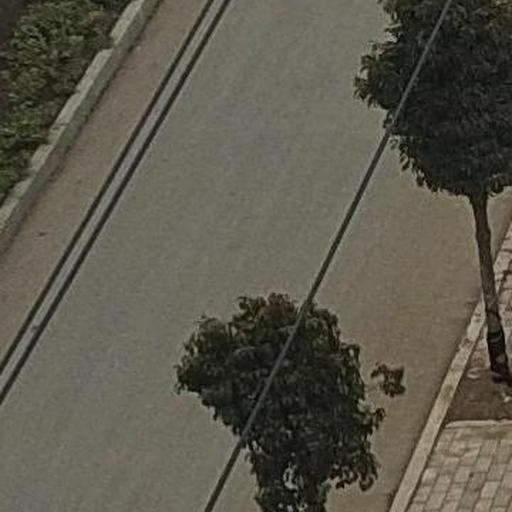
\includegraphics[width = 1.65in]{imgs/pldu_base_imgs/250.jpg}} &
%   \subfloat{
\includegraphics[width = 1.65in]{imgs/pldu_gt/250.png}} &
%   \subfloat{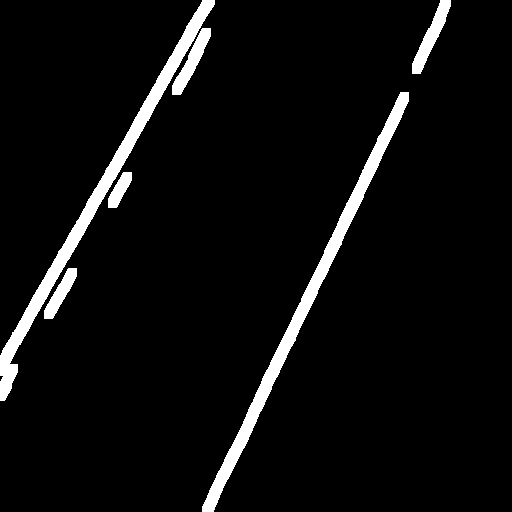
\includegraphics[width = 1.65in]{imgs/pldu_old/250.png}} &
%   \subfloat{
\includegraphics[width = 1.65in]{imgs/pldu_new/250.png}}\\
%   \subfloat{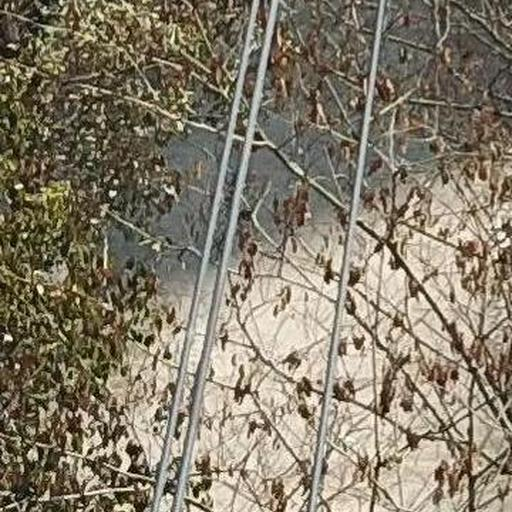
\includegraphics[width = 1.65in]{imgs/pldu_base_imgs/355.jpg}} &
%   \subfloat{
\includegraphics[width = 1.65in]{imgs/pldu_gt/355.png}} &
%   \subfloat{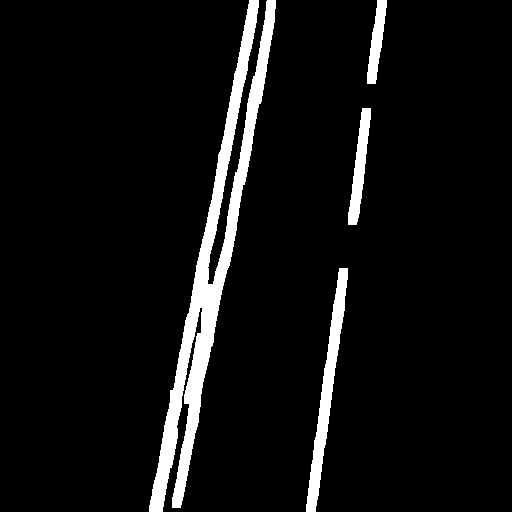
\includegraphics[width = 1.65in]{imgs/pldu_old/355.png}} &
%   \subfloat{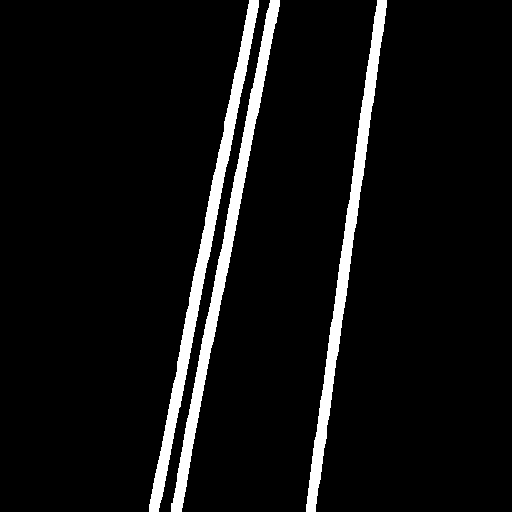
\includegraphics[width = 1.65in]{imgs/pldu_new/355.png}}\\
%   % \subfloat{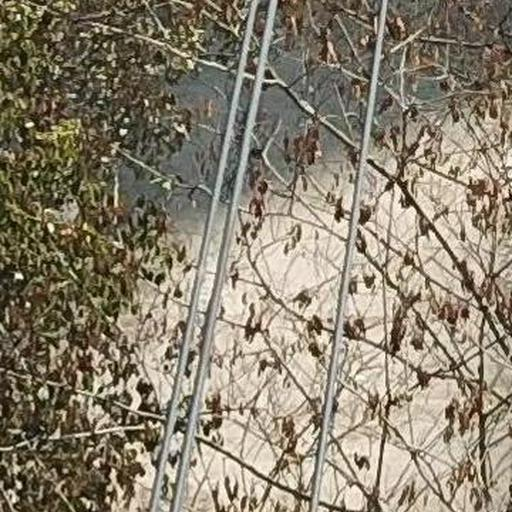
\includegraphics[width = 1.65in]{imgs/pldu_base_imgs/358.jpg}} &
%   % \subfloat{
\includegraphics[width = 1.65in]{imgs/pldu_gt/358.png}} &
%   % \subfloat{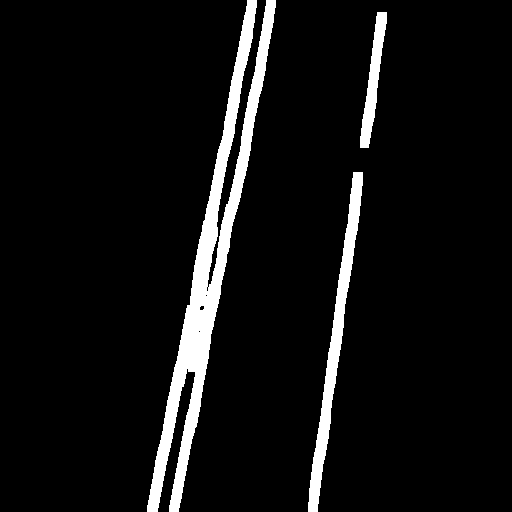
\includegraphics[width = 1.65in]{imgs/pldu_old/358.png}} &
%   % \subfloat{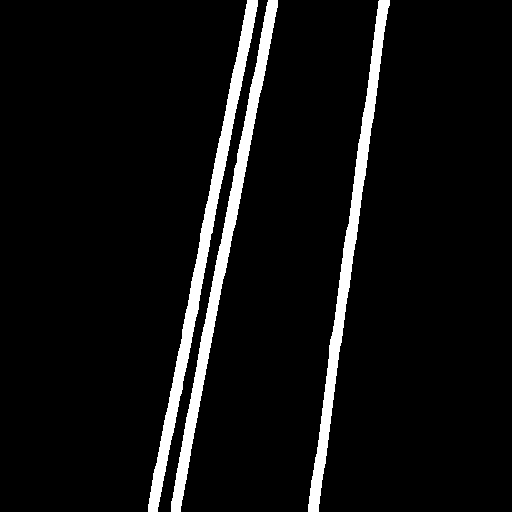
\includegraphics[width = 1.65in]{imgs/pldu_new/358.png}}\\
%   \subfloat{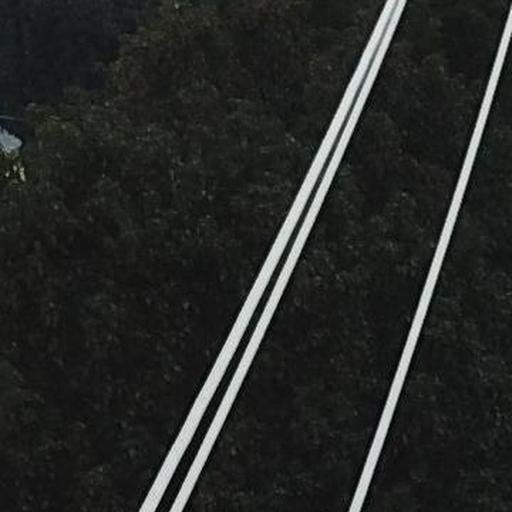
\includegraphics[width = 1.65in]{imgs/pldu_base_imgs/481.jpg}} &
%   \subfloat{
\includegraphics[width = 1.65in]{imgs/pldu_gt/481.png}} &
%   \subfloat{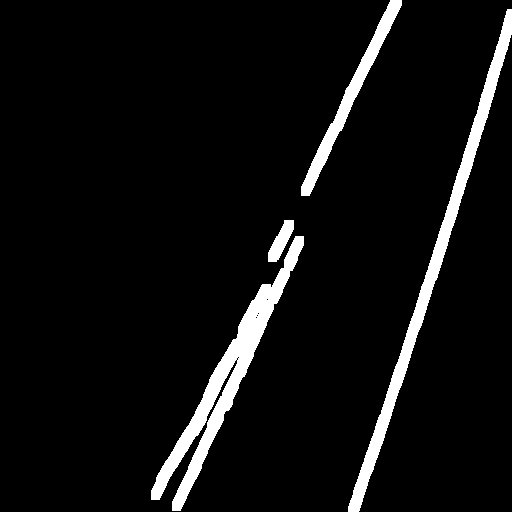
\includegraphics[width = 1.65in]{imgs/pldu_old/481.png}} &
%   \subfloat{
\includegraphics[width = 1.65in]{imgs/pldu_new/481.png}}\\
%   \subfloat{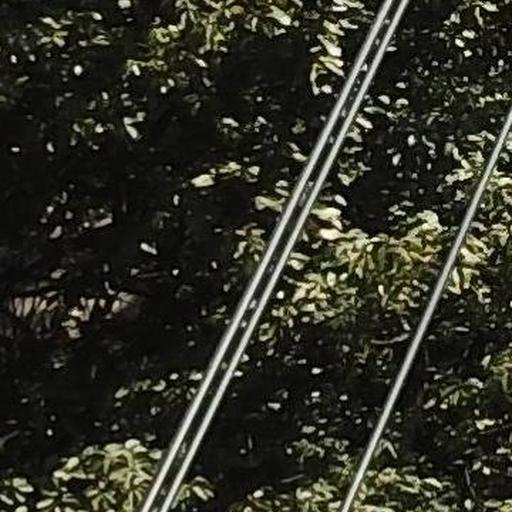
\includegraphics[width = 1.65in]{imgs/pldu_base_imgs/426.jpg}} &
%   \subfloat{
\includegraphics[width = 1.65in]{imgs/pldu_gt/426.png}} &
%   \subfloat{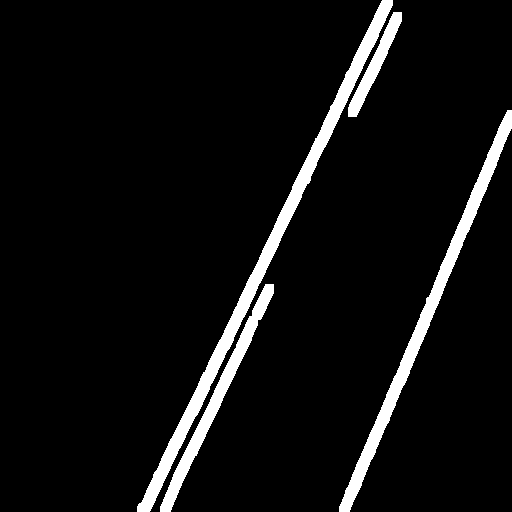
\includegraphics[width = 1.65in]{imgs/pldu_old/426.png}} &
%   \subfloat{
\includegraphics[width = 1.65in]{imgs/pldu_new/426.png}}\\
%   \subfloat{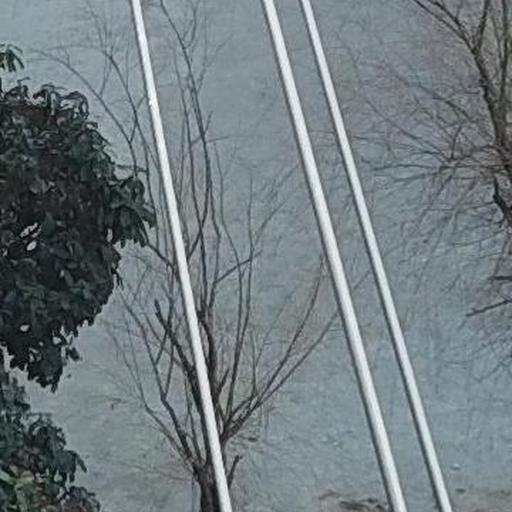
\includegraphics[width = 1.65in]{imgs/pldu_base_imgs/637.jpg}} &
%   \subfloat{
\includegraphics[width = 1.65in]{imgs/pldu_gt/637.png}} &
%   \subfloat{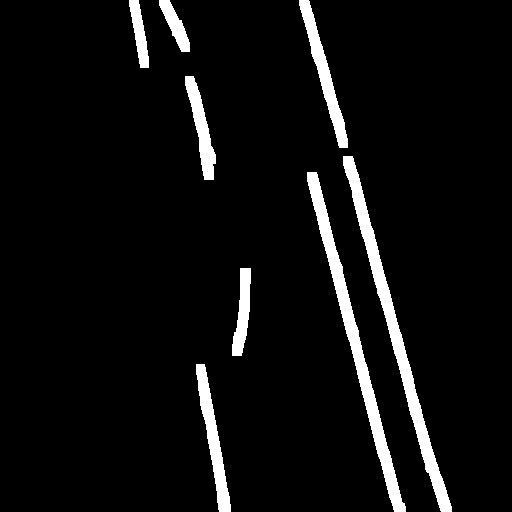
\includegraphics[width = 1.65in]{imgs/pldu_old/637.png}} &
%   \subfloat{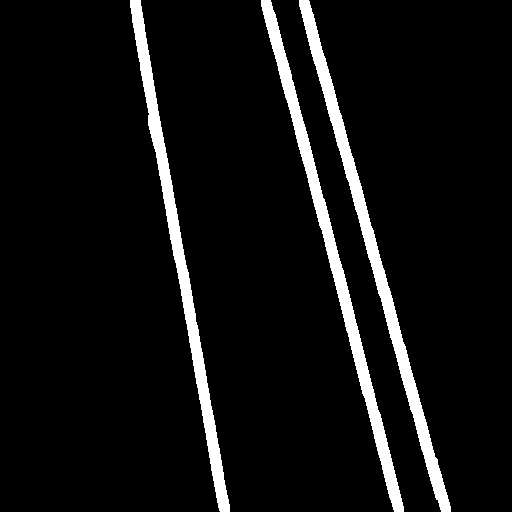
\includegraphics[width = 1.65in]{imgs/pldu_new/637.png}}\\

%   % Add caption row
%   Image & Ground truth & LSNet & LSNetv2
%   % \subfloat[caption]{\includegraphics[width = 1.5in]{something}}\\
%   \end{tabularx}
%   \caption{\label{PLDU_example}Example test results of LSNet and LSNetv2 on test images in PLDU dataset. The columns from left to right contain: original images, ground truth segment map, outputs of LSNet and outputs of LSNetv2}
% \end{figure*}

\begin{figure*}
  \addtolength{\tabcolsep}{-5pt} 
  \begin{tabularx}{\textwidth}{ccccc}
  \centering
  \subfloat{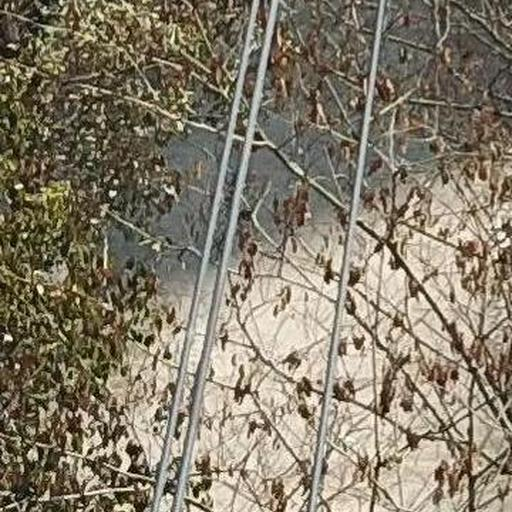
\includegraphics[width = 1.40in]{imgs/pldu_base_imgs/355.jpg}} &
  \subfloat{
\includegraphics[width = 1.40in]{imgs/pldu_gt/355.png}} &
  \subfloat{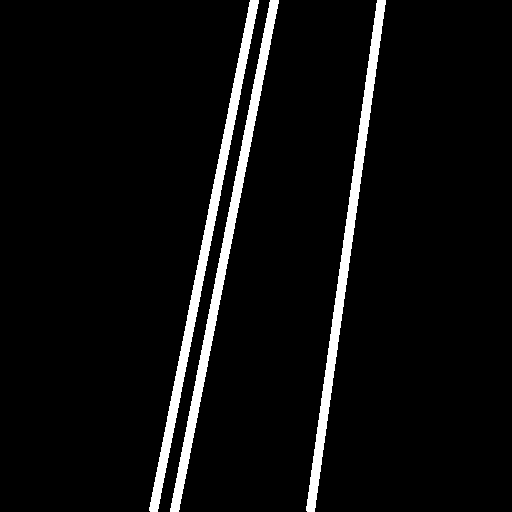
\includegraphics[width = 1.40in]{imgs/hawp/pldu_ha/355.png}} &
  \subfloat{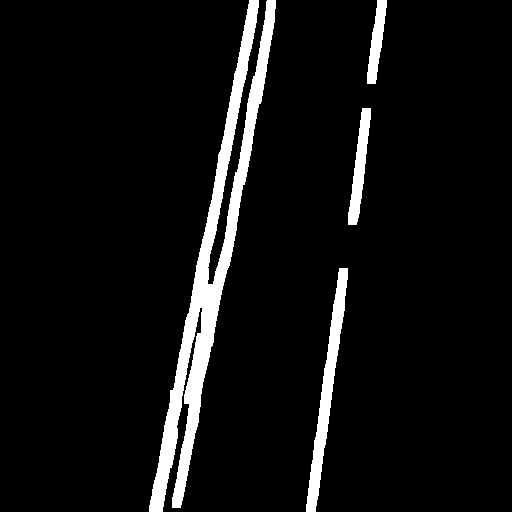
\includegraphics[width = 1.40in]{imgs/pldu_old/355.png}} &
  \subfloat{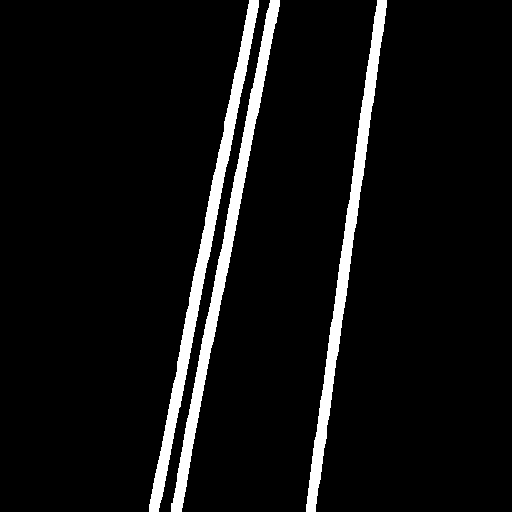
\includegraphics[width = 1.40in]{imgs/pldu_new/355.png}} \\
  \subfloat{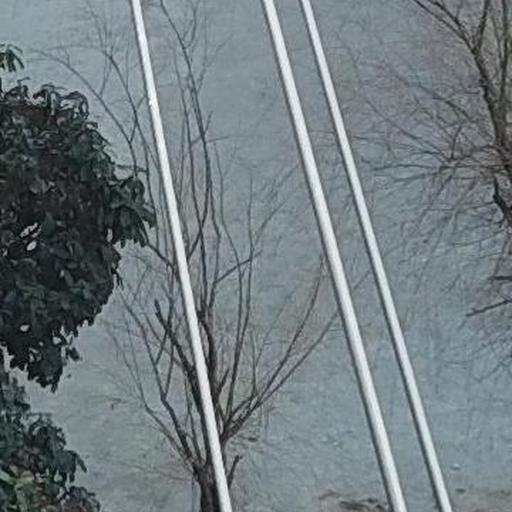
\includegraphics[width = 1.40in]{imgs/pldu_base_imgs/637.jpg}} &
  \subfloat{
\includegraphics[width = 1.40in]{imgs/pldu_gt/637.png}} &
  \subfloat{
\includegraphics[width = 1.40in]{imgs/hawp/pldu_ha/637.png}} &
  \subfloat{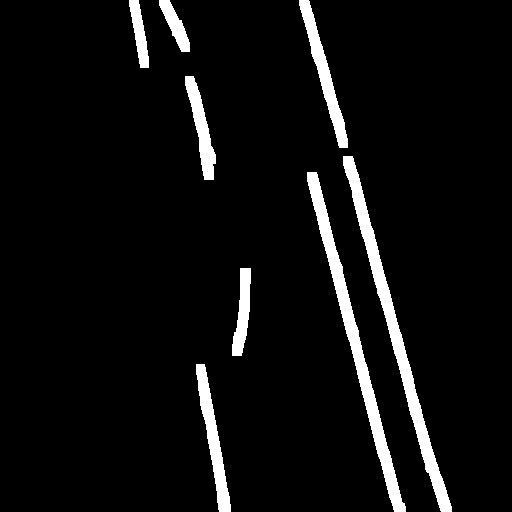
\includegraphics[width = 1.40in]{imgs/pldu_old/637.png}} &
  \subfloat{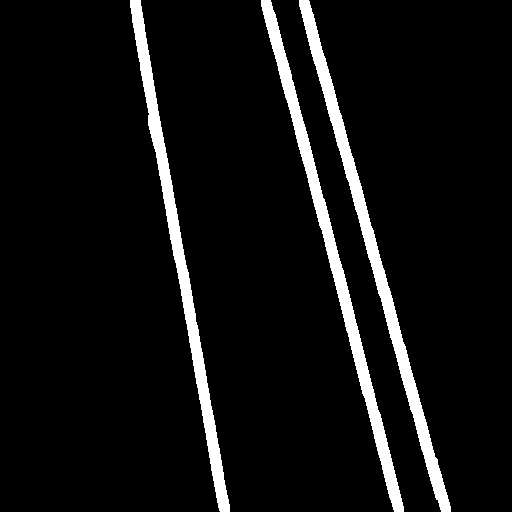
\includegraphics[width = 1.40in]{imgs/pldu_new/637.png}} \\
  \subfloat{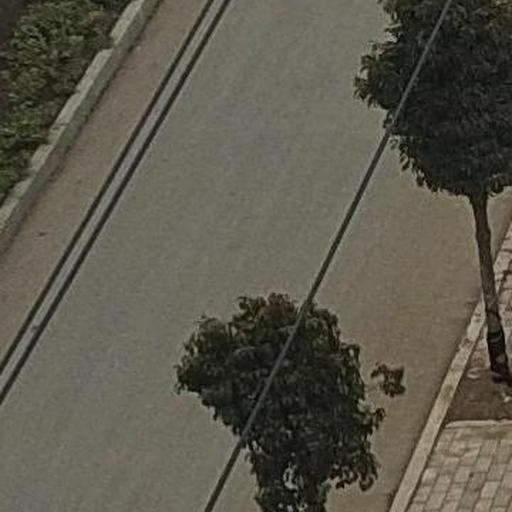
\includegraphics[width = 1.40in]{imgs/pldu_base_imgs/250.jpg}} &
  \subfloat{
\includegraphics[width = 1.40in]{imgs/pldu_gt/250.png}} &
  \subfloat{
\includegraphics[width = 1.40in]{imgs/hawp/pldu_ha/250.png}} &
  \subfloat{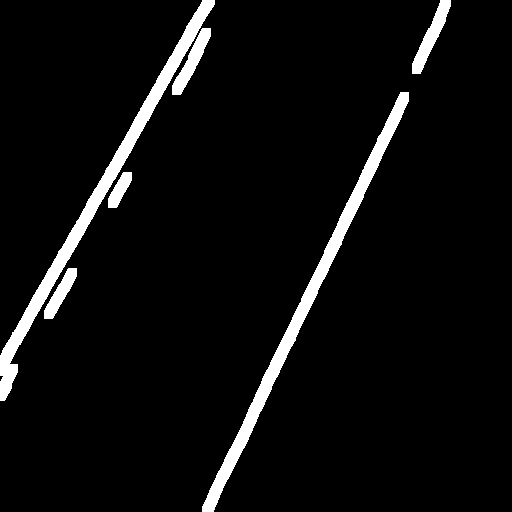
\includegraphics[width = 1.40in]{imgs/pldu_old/250.png}} &
  \subfloat{
\includegraphics[width = 1.40in]{imgs/pldu_new/250.png}} \\
  \subfloat{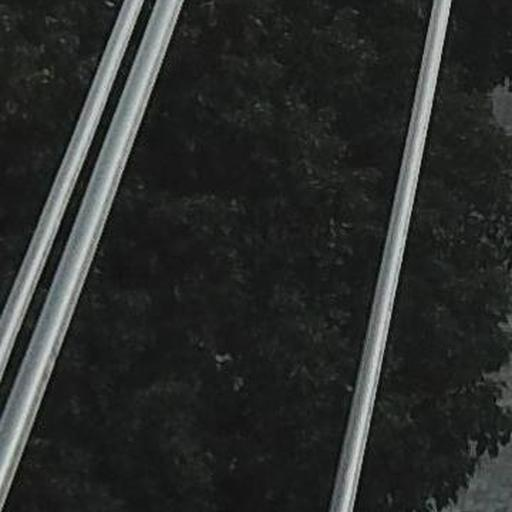
\includegraphics[width = 1.40in]{imgs/pldu_base_imgs/510.jpg}} &
  \subfloat{
\includegraphics[width = 1.40in]{imgs/pldu_gt/510.png}} &
  \subfloat{
\includegraphics[width = 1.40in]{imgs/hawp/pldu_ha/510.png}} &
  \subfloat{
\includegraphics[width = 1.40in]{imgs/pldu_old/510.png}} &
  \subfloat{
\includegraphics[width = 1.40in]{imgs/pldu_new/510.png}} \\
  \subfloat{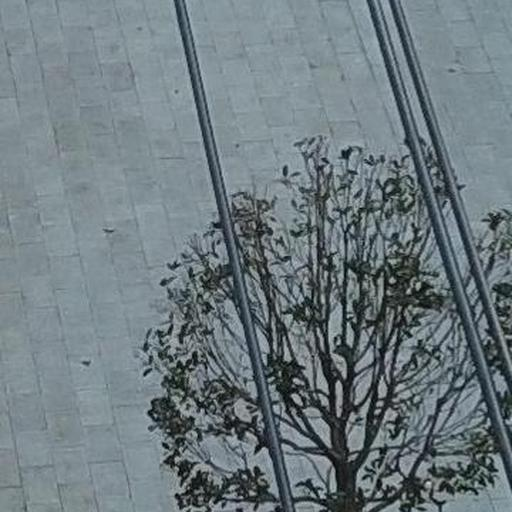
\includegraphics[width = 1.40in]{imgs/pldu_base_imgs/409.jpg}} &
  \subfloat{
\includegraphics[width = 1.40in]{imgs/pldu_gt/409.png}} &
  \subfloat{\includegraphics[width = 1.40in]{imgs/hawp/pldu_ha/409.png}} &
  \subfloat{\includegraphics[width = 1.40in]{imgs/pldu_old/409.png}} &
  \subfloat{\includegraphics[width = 1.40in]{imgs/pldu_new/409.png}} \\
  \subfloat{\includegraphics[width = 1.40in]{imgs/pldu_base_imgs/481.jpg}} &
  \subfloat{\includegraphics[width = 1.40in]{imgs/pldu_gt/481.png}} &
  \subfloat{\includegraphics[width = 1.40in]{imgs/hawp/pldu_ha/481.png}} &
  \subfloat{\includegraphics[width = 1.40in]{imgs/pldu_old/481.png}} &
  \subfloat{\includegraphics[width = 1.40in]{imgs/pldu_new/481.png}}\\
  % \subfloat{\includegraphics[width = 265in]{imgs/pldu_base_imgs/358.jpg}} &
  % \subfloat{\includegraphics[width = 265in]{imgs/pldu_gt/358.png}} &
  % \subfloat{\includegraphics[width = 265in]{imgs/pldu_old/358.png}} &
  % \subfloat{\includegraphics[width = 265in]{imgs/pldu_new/358.png}}\\
  

  % Add caption row
  Image & Ground truth & LSNet & LSNetv2
  % \subfloat[caption]{\includegraphics[width = 1.5in]{something}}\\
  \end{tabularx}
  \caption{\label{PLDU_example}Example test results of LSNet and LSNetv2 on test images in PLDU dataset. The columns from left to right contain: original images, ground truth segment map, outputs of LSNet and outputs of LSNetv2}
\end{figure*}

\begin{figure*}
  \addtolength{\tabcolsep}{-5pt} 
  \begin{tabularx}{\textwidth}{ccccc}
  \centering
  \subfloat{\includegraphics[width = 1.40in]{imgs/pldm_base_imgs/18.jpg}} &
  \subfloat{\includegraphics[width = 1.40in]{imgs/pldm_gt/18.png}} &
  \subfloat{\includegraphics[width = 1.40in]{imgs/hawp/pldm_ha/18.png}} &
  \subfloat{\includegraphics[width = 1.40in]{imgs/pldm_old/18.png}} &
  \subfloat{\includegraphics[width = 1.40in]{imgs/pldm_new/18.png}} \\
  \subfloat{\includegraphics[width = 1.40in]{imgs/pldm_base_imgs/4.jpg}} &
  \subfloat{\includegraphics[width = 1.40in]{imgs/pldm_gt/4.png}} &
  \subfloat{\includegraphics[width = 1.40in]{imgs/hawp/pldm_ha/4.png}} &
  \subfloat{\includegraphics[width = 1.40in]{imgs/pldm_old/4.png}} &
  \subfloat{\includegraphics[width = 1.40in]{imgs/pldm_new/4.png}} \\
  \subfloat{\includegraphics[width = 1.40in]{imgs/pldm_base_imgs/24.jpg}} &
  \subfloat{\includegraphics[width = 1.40in]{imgs/pldm_gt/24.png}} &
  \subfloat{\includegraphics[width = 1.40in]{imgs/hawp/pldm_ha/24.png}} &
  \subfloat{\includegraphics[width = 1.40in]{imgs/pldm_old/24.png}} &
  \subfloat{\includegraphics[width = 1.40in]{imgs/pldm_new/24.png}} \\
  \subfloat{\includegraphics[width = 1.40in]{imgs/pldm_base_imgs/124.jpg}} &
  \subfloat{\includegraphics[width = 1.40in]{imgs/pldm_gt/124.png}} &
  \subfloat{\includegraphics[width = 1.40in]{imgs/hawp/pldm_ha/124.png}} &
  \subfloat{\includegraphics[width = 1.40in]{imgs/pldm_old/124.png}} &
  \subfloat{\includegraphics[width = 1.40in]{imgs/pldm_new/124.png}} \\

  % Add caption row
  % \subfloat[caption]{\includegraphics[width = 1.5in]{something}}\\
  \end{tabularx}
  \caption{\label{PLDM_example}Example test results of LSNet and LSNetv2 on test images in PLDM dataset. The columns from left to right contain: original images, ground truth segment map, outputs of LSNet and outputs of LSNetv2}
\end{figure*}

\begin{table}[]
\begin{tabular}{lll|ll|ll|ll}
               & \multicolumn{2}{l|}{PLDU}    & \multicolumn{2}{l|}{PLDM}    & \multicolumn{2}{l|}{TTPLA}   & \multicolumn{2}{l}{Esmart}   \\ \cline{2-9} 
               & line width & score threshold & line width & score threshold & line width & score threshold & line width & score threshold \\ \hline
Best $F_1$     & 7          & 0.8             & 7          & 0.2             & 2          & 0.2             & 5          & 0.1             \\
Best $F_\beta$ & 7          & 0.1             & 3          & 0.3             & 2          & 0.7             & 5          & 0.4             \\ \hline
\end{tabular}
\caption{\label{hawp_prop} Properties}
\end{table}

\begin{figure*}
  \addtolength{\tabcolsep}{-5pt} 
  \begin{tabularx}{\textwidth}{ccccc}
  \centering
  \subfloat{\includegraphics[width = 1.40in]{imgs/ttpla_base_imgs/107_1410_2.jpg}} &
  \subfloat{\includegraphics[width = 1.40in]{imgs/ttpla_gt/107_1410_2.png}} &
  \subfloat{\includegraphics[width = 1.40in]{imgs/hawp/ttpla_ha/107_1410_2.png}} &
  \subfloat{\includegraphics[width = 1.40in]{imgs/ttpla_old/107_1410_2.png}} &
  \subfloat{\includegraphics[width = 1.40in]{imgs/ttpla_new/107_1410_2.png}} \\
  \subfloat{\includegraphics[width = 1.40in]{imgs/ttpla_base_imgs/25_00272_1.jpg}} &
  \subfloat{\includegraphics[width = 1.40in]{imgs/ttpla_gt/25_00272_1.png}} &
  \subfloat{\includegraphics[width = 1.40in]{imgs/hawp/ttpla_ha/25_00272_1.png}} &
  \subfloat{\includegraphics[width = 1.40in]{imgs/ttpla_old/25_00272_1.png}} &
  \subfloat{\includegraphics[width = 1.40in]{imgs/ttpla_new/25_00272_1.png}} \\
  % \subfloat{\includegraphics[width = 1.40in]{imgs/ttpla_base_imgs/14_00486_2.jpg}} &
  % \subfloat{\includegraphics[width = 1.40in]{imgs/ttpla_gt/14_00486_2.png}} &
  % \subfloat{\includegraphics[width = 1.40in]{imgs/hawp/ttpla_ha/14_00486_2.png}} &
  % \subfloat{\includegraphics[width = 1.40in]{imgs/ttpla_old/14_00486_2.png}} &
  % \subfloat{\includegraphics[width = 1.40in]{imgs/ttpla_new/14_00486_2.png}} \\
  \subfloat{\includegraphics[width = 1.40in]{imgs/ttpla_base_imgs/23_00706_2.jpg}}&
  \subfloat{\includegraphics[width = 1.40in]{imgs/ttpla_gt/23_00706_2.png}}&
  \subfloat{\includegraphics[width = 1.40in]{imgs/hawp/ttpla_ha/23_00706_2.png}}&
  \subfloat{\includegraphics[width = 1.40in]{imgs/ttpla_old/23_00706_2.png}}&
  \subfloat{\includegraphics[width = 1.40in]{imgs/ttpla_new/23_00706_2.png}}\\

  \subfloat{\includegraphics[width = 1.40in]{imgs/ttpla_base_imgs/110_0_1.jpg}}&
  \subfloat{\includegraphics[width = 1.40in]{imgs/ttpla_gt/110_0_1.png}}&
  \subfloat{\includegraphics[width = 1.40in]{imgs/hawp/ttpla_ha/110_0_1.png}}&
  \subfloat{\includegraphics[width = 1.40in]{imgs/ttpla_old/110_0_1.png}}&
  \subfloat{\includegraphics[width = 1.40in]{imgs/ttpla_new/110_0_1.png}}\\
  \subfloat{\includegraphics[width = 1.40in]{imgs/ttpla_base_imgs/25_00667_2.jpg}}&
  \subfloat{\includegraphics[width = 1.40in]{imgs/ttpla_gt/25_00667_2.png}}&
  \subfloat{\includegraphics[width = 1.40in]{imgs/hawp/ttpla_ha/25_00667_2.png}}&
  \subfloat{\includegraphics[width = 1.40in]{imgs/ttpla_old/25_00667_2.png}}&
  \subfloat{\includegraphics[width = 1.40in]{imgs/ttpla_new/25_00667_2.png}}\\
  \subfloat{\includegraphics[width = 1.40in]{imgs/ttpla_base_imgs/42_00551_1.jpg}}&
  \subfloat{\includegraphics[width = 1.40in]{imgs/ttpla_gt/42_00551_1.png}}&
  \subfloat{\includegraphics[width = 1.40in]{imgs/hawp/ttpla_ha/42_00551_1.png}}&
  \subfloat{\includegraphics[width = 1.40in]{imgs/ttpla_old/42_00551_1.png}}&
  \subfloat{\includegraphics[width = 1.40in]{imgs/ttpla_new/42_00551_1.png}}\\
  
  % \subfloat{\includegraphics[width = 1.65in]{imgs/ttpla_base_imgs/25_00272_1.jpg}} &
  % \subfloat{\includegraphics[width = 1.65in]{imgs/ttpla_gt/25_00272_1.png}} &
  % \subfloat{\includegraphics[width = 1.65in]{imgs/ttpla_old/25_00272_1.png}} &
  % \subfloat{\includegraphics[width = 1.65in]{imgs/ttpla_new/25_00272_1.png}}\\

  % Add caption row
  Image & Ground truth & HAWPv2 & LSNet & LSNetv2
  % \subfloat[caption]{\includegraphics[width = 1.5in]{something}}\\
  \end{tabularx}
  \caption{\label{ttpla_example_0}First five example test results of LSNet and LSNetv2 on test images in PLDU dataset. The columns from left to right contain: original images, ground truth segment map, outputs of LSNet and outputs of LSNetv2}
\end{figure*}

% \begin{figure*}
%   \begin{tabularx}{\textwidth}{cccc}
%   \centering
%   \subfloat{\includegraphics[width = 1.65in]{imgs/ttpla_base_imgs/25_00667_2.jpg}} &
%   \subfloat{\includegraphics[width = 1.65in]{imgs/ttpla_base_imgs/33_7545_1.jpg}} &
%   \subfloat{\includegraphics[width = 1.65in]{imgs/ttpla_base_imgs/42_00551_1.jpg}} &
%   \subfloat{\includegraphics[width = 1.65in]{imgs/ttpla_base_imgs/47_00101_1.jpg}}\\
%   \subfloat{\includegraphics[width = 1.65in]{imgs/ttpla_gt/25_00667_2.png}} &
%   \subfloat{\includegraphics[width = 1.65in]{imgs/ttpla_gt/33_7545_1.png}} &
%   \subfloat{\includegraphics[width = 1.65in]{imgs/ttpla_gt/42_00551_1.png}} &
%   \subfloat{\includegraphics[width = 1.65in]{imgs/ttpla_gt/47_00101_1.png}}\\
%   \subfloat{\includegraphics[width = 1.65in]{imgs/hawp/ttpla_ha/25_00667_2.png}} &
%   \subfloat{\includegraphics[width = 1.65in]{imgs/hawp/ttpla_ha/33_7545_1.png}} &
%   \subfloat{\includegraphics[width = 1.65in]{imgs/hawp/ttpla_ha/42_00551_1.png}} &
%   \subfloat{\includegraphics[width = 1.65in]{imgs/hawp/ttpla_ha/47_00101_1.png}}\\
%   \subfloat{\includegraphics[width = 1.65in]{imgs/ttpla_old/25_00667_2.png}} &
%   \subfloat{\includegraphics[width = 1.65in]{imgs/ttpla_old/33_7545_1.png}} &
%   \subfloat{\includegraphics[width = 1.65in]{imgs/ttpla_old/42_00551_1.png}} &
%   \subfloat{\includegraphics[width = 1.65in]{imgs/ttpla_old/47_00101_1.png}}\\
%   \subfloat{\includegraphics[width = 1.65in]{imgs/ttpla_new/25_00667_2.png}} &
%   \subfloat{\includegraphics[width = 1.65in]{imgs/ttpla_new/33_7545_1.png}} &
%   \subfloat{\includegraphics[width = 1.65in]{imgs/ttpla_new/42_00551_1.png}} &
%   \subfloat{\includegraphics[width = 1.65in]{imgs/ttpla_new/47_00101_1.png}}\\
%   % \subfloat{\includegraphics[width = 1.65in]{imgs/ttpla_base_imgs/57_00141_2.jpg}} &
%   % \subfloat{\includegraphics[width = 1.65in]{imgs/ttpla_gt/57_00141_2.png}} &
%   % \subfloat{\includegraphics[width = 1.65in]{imgs/ttpla_old/57_00141_2.png}} &
%   % \subfloat{\includegraphics[width = 1.65in]{imgs/ttpla_new/57_00141_2.png}}\\
%   % \subfloat[caption]{\includegraphics[width = 1.5in]{something}}\\
%   \end{tabularx}
%   \caption{\label{ttpla_example_1}Second five example test results of LSNet and LSNetv2 on test images in PLDU dataset. The columns from left to right contain: original images, ground truth segment map, outputs of LSNet and outputs of LSNetv2}
% \end{figure*}

% \begin{figure*}
%   \begin{tabularx}{\textwidth}{ccccc}
%   \centering
%   \subfloat{\includegraphics[width = 1.65in]{imgs/ttpla_base_imgs/110_0_1.jpg}} &
%   \subfloat{\includegraphics[width = 1.65in]{imgs/ttpla_base_imgs/57_00141_2.jpg}}\\
%   \subfloat{\includegraphics[width = 1.65in]{imgs/ttpla_gt/110_0_1.png}} &
%   \subfloat{\includegraphics[width = 1.65in]{imgs/ttpla_gt/57_00141_2.png}}\\
%   \subfloat{\includegraphics[width = 1.65in]{imgs/hawp/ttpla_ha/110_0_1.png}} &
%   \subfloat{\includegraphics[width = 1.65in]{imgs/hawp/ttpla_ha/57_00141_2.png}}\\
%   \subfloat{\includegraphics[width = 1.65in]{imgs/ttpla_old/110_0_1.png}} &
%   \subfloat{\includegraphics[width = 1.65in]{imgs/ttpla_old/57_00141_2.png}}\\
%   \subfloat{\includegraphics[width = 1.65in]{imgs/ttpla_new/110_0_1.png}} &
%   \subfloat{\includegraphics[width = 1.65in]{imgs/ttpla_new/57_00141_2.png}}\\
%   \end{tabularx}
%   \caption{\label{ttpla_example_1}Second five example test results of LSNet and LSNetv2 on test images in PLDU dataset. The columns from left to right contain: original images, ground truth segment map, outputs of LSNet and outputs of LSNetv2}
% \end{figure*}




\begin{figure*}
  \addtolength{\tabcolsep}{-5pt} 
  \begin{tabularx}{\textwidth}{ccccc}
  \centering 
  % \subfloat{\includegraphics[width = 1.40in]{imgs/esmart_base_imgs/Alta__4ba599e9-bf87-4283-aa2c-8d0bdd9b4e6e.JPG}} &
  % \subfloat{\includegraphics[width = 1.40in]{imgs/esmart_gt/Alta__4ba599e9-bf87-4283-aa2c-8d0bdd9b4e6e.png}} &
  % \subfloat{\includegraphics[width = 1.40in]{imgs/hawp/esmart_ha/Alta__4ba599e9-bf87-4283-aa2c-8d0bdd9b4e6e.png}} &
  % \subfloat{\includegraphics[width = 1.40in]{imgs/esmart_old/Alta__4ba599e9-bf87-4283-aa2c-8d0bdd9b4e6e.png}} &
  % \subfloat{\includegraphics[width = 1.40in]{imgs/esmart_new/Alta__4ba599e9-bf87-4283-aa2c-8d0bdd9b4e6e.png}} \\
  \subfloat{\includegraphics[width = 1.40in]{imgs/esmart_base_imgs/Alta__6a6a5379-a993-4be1-9d79-236991f70d38.JPG}} &
  \subfloat{\includegraphics[width = 1.40in]{imgs/esmart_gt/Alta__6a6a5379-a993-4be1-9d79-236991f70d38.png}} &
  \subfloat{\includegraphics[width = 1.40in]{imgs/hawp/esmart_ha/Alta__6a6a5379-a993-4be1-9d79-236991f70d38.png}} &
  \subfloat{\includegraphics[width = 1.40in]{imgs/esmart_old/Alta__6a6a5379-a993-4be1-9d79-236991f70d38.png}} &
  \subfloat{\includegraphics[width = 1.40in]{imgs/esmart_new/Alta__6a6a5379-a993-4be1-9d79-236991f70d38.png}} \\
  \subfloat{\includegraphics[width = 1.40in]{imgs/esmart_base_imgs/Alta__05ceb653-bdc2-78a8-0747-a63831e3ebc9.JPG}} &
  \subfloat{\includegraphics[width = 1.40in]{imgs/esmart_gt/Alta__05ceb653-bdc2-78a8-0747-a63831e3ebc9.png}} &
  \subfloat{\includegraphics[width = 1.40in]{imgs/hawp/esmart_ha/Alta__05ceb653-bdc2-78a8-0747-a63831e3ebc9.png}} &
  \subfloat{\includegraphics[width = 1.40in]{imgs/esmart_old/Alta__05ceb653-bdc2-78a8-0747-a63831e3ebc9.png}} &
  \subfloat{\includegraphics[width = 1.40in]{imgs/esmart_new/Alta__05ceb653-bdc2-78a8-0747-a63831e3ebc9.png}} \\
  \subfloat{\includegraphics[width = 1.40in]{imgs/esmart_base_imgs/Dalane__Dalane+IA__DAT_7909.JPG}} &
  \subfloat{\includegraphics[width = 1.40in]{imgs/esmart_gt/Dalane__Dalane+IA__DAT_7909.png}} &
  \subfloat{\includegraphics[width = 1.40in]{imgs/hawp/esmart_ha/Dalane__Dalane+IA__DAT_7909.png}} &
  \subfloat{\includegraphics[width = 1.40in]{imgs/esmart_old/Dalane__Dalane+IA__DAT_7909.png}} &
  \subfloat{\includegraphics[width = 1.40in]{imgs/esmart_new/Dalane__Dalane+IA__DAT_7909.png}}\\
  
  \subfloat{\includegraphics[width = 1.40in]{imgs/esmart_base_imgs/Alta__bbbc763d-c6c4-4ab9-0b9b-9e0307a872ae.JPG}} &
  \subfloat{\includegraphics[width = 1.40in]{imgs/esmart_gt/Alta__bbbc763d-c6c4-4ab9-0b9b-9e0307a872ae.png}} &
  \subfloat{\includegraphics[width = 1.40in]{imgs/hawp/esmart_ha/Alta__bbbc763d-c6c4-4ab9-0b9b-9e0307a872ae.png}} &
  \subfloat{\includegraphics[width = 1.40in]{imgs/esmart_old/Alta__bbbc763d-c6c4-4ab9-0b9b-9e0307a872ae.png}} &
  \subfloat{\includegraphics[width = 1.40in]{imgs/esmart_new/Alta__bbbc763d-c6c4-4ab9-0b9b-9e0307a872ae.png}} \\
  \subfloat{\includegraphics[width = 1.40in]{imgs/esmart_base_imgs/Alta__cf519095-8e39-35eb-448d-1cd731af29b1.JPG}} &
  \subfloat{\includegraphics[width = 1.40in]{imgs/esmart_gt/Alta__cf519095-8e39-35eb-448d-1cd731af29b1.png}} &
  \subfloat{\includegraphics[width = 1.40in]{imgs/hawp/esmart_ha/Alta__cf519095-8e39-35eb-448d-1cd731af29b1.png}} &
  \subfloat{\includegraphics[width = 1.40in]{imgs/esmart_old/Alta__cf519095-8e39-35eb-448d-1cd731af29b1.png}} &
  \subfloat{\includegraphics[width = 1.40in]{imgs/esmart_new/Alta__cf519095-8e39-35eb-448d-1cd731af29b1.png}} \\
  \subfloat{\includegraphics[width = 1.40in]{imgs/esmart_base_imgs/Haugaland__Haugaland+Opptrening__Helikopterbilder+2011___DSC0539.JPG}} &
  \subfloat{\includegraphics[width = 1.40in]{imgs/esmart_gt/Haugaland__Haugaland+Opptrening__Helikopterbilder+2011___DSC0539.png}} &
  \subfloat{\includegraphics[width = 1.40in]{imgs/hawp/esmart_ha/Haugaland__Haugaland+Opptrening__Helikopterbilder+2011___DSC0539.png}} &
  \subfloat{\includegraphics[width = 1.40in]{imgs/esmart_old/Haugaland__Haugaland+Opptrening__Helikopterbilder+2011___DSC0539.png}} &
  \subfloat{\includegraphics[width = 1.40in]{imgs/esmart_new/Haugaland__Haugaland+Opptrening__Helikopterbilder+2011___DSC0539.png}} \\
  % \subfloat{\includegraphics[width = 1.65in]{imgs/esmart_base_imgs/Alta__6a6a5379-a993-4be1-9d79-236991f70d38.JPG}} &
  % \subfloat{\includegraphics[width = 1.65in]{imgs/esmart_base_imgs/Alta__9abf75f2-84d8-490d-9a2e-ae77606bcd02.JPG}}\\
  % \subfloat{\includegraphics[width = 1.65in]{imgs/esmart_gt/Alta__6a6a5379-a993-4be1-9d79-236991f70d38.png}} &
  % \subfloat{\includegraphics[width = 1.65in]{imgs/esmart_gt/Alta__9abf75f2-84d8-490d-9a2e-ae77606bcd02.png}}\\
  % \subfloat{\includegraphics[width = 1.65in]{imgs/hawp/esmart_ha/Alta__6a6a5379-a993-4be1-9d79-236991f70d38.png}} &
  % \subfloat{\includegraphics[width = 1.65in]{imgs/hawp/esmart_ha/Alta__9abf75f2-84d8-490d-9a2e-ae77606bcd02.png}}\\
  % \subfloat{\includegraphics[width = 1.65in]{imgs/esmart_old/Alta__6a6a5379-a993-4be1-9d79-236991f70d38.png}} &
  % \subfloat{\includegraphics[width = 1.65in]{imgs/esmart_old/Alta__9abf75f2-84d8-490d-9a2e-ae77606bcd02.png}}\\
  % \subfloat{\includegraphics[width = 1.65in]{imgs/esmart_new/Alta__6a6a5379-a993-4be1-9d79-236991f70d38.png}} &
  % \subfloat{\includegraphics[width = 1.65in]{imgs/esmart_new/Alta__9abf75f2-84d8-490d-9a2e-ae77606bcd02.png}}\\
  % \subfloat{\includegraphics[width = 1.65in]{imgs/esmart_base_imgs/Alta__98d795b2-512d-e740-2b9c-dfb9b6b40696.JPG}} &
  % \subfloat{\includegraphics[width = 1.65in]{imgs/esmart_gt/Alta__98d795b2-512d-e740-2b9c-dfb9b6b40696.png}} &
  % \subfloat{\includegraphics[width = 1.65in]{imgs/esmart_old/Alta__98d795b2-512d-e740-2b9c-dfb9b6b40696.png}} &
  % \subfloat{\includegraphics[width = 1.65in]{imgs/esmart_new/Alta__98d795b2-512d-e740-2b9c-dfb9b6b40696.png}}\\

  % Add caption row
  Image & Ground truth & LSNet & LSNetv2
  % \subfloat[caption]{\includegraphics[width = 1.5in]{something}}\\
  \end{tabularx}
  \caption{\label{esmart_example_0}Example test results of LSNet and LSNetv2 on test images in Esmart dataset. The columns from left to right contain: original images, ground truth segment map, outputs of LSNet and outputs of LSNetv2}
\end{figure*}

% \begin{figure*}
%   \begin{tabularx}{\textwidth}{cccc}
%   \centering
%   \subfloat{\includegraphics[width = 1.65in]{imgs/esmart_base_imgs/Alta__a1cf5776-0454-4ef6-8726-ad25b0023293.JPG}} &
%   \subfloat{\includegraphics[width = 1.65in]{imgs/esmart_base_imgs/Alta__bbbc763d-c6c4-4ab9-0b9b-9e0307a872ae.JPG}} &
%   \subfloat{\includegraphics[width = 1.65in]{imgs/esmart_base_imgs/Dalane__Dalane+IA__DAT_7559.JPG}} &
%   \subfloat{\includegraphics[width = 1.65in]{imgs/esmart_base_imgs/Dalane__Dalane+IA__DAT_6749.JPG}}\\
%   \subfloat{\includegraphics[width = 1.65in]{imgs/esmart_gt/Alta__a1cf5776-0454-4ef6-8726-ad25b0023293.png}} &
%   \subfloat{\includegraphics[width = 1.65in]{imgs/esmart_gt/Alta__bbbc763d-c6c4-4ab9-0b9b-9e0307a872ae.png}} &
%   \subfloat{\includegraphics[width = 1.65in]{imgs/esmart_gt/Dalane__Dalane+IA__DAT_7559.png}} &
%   \subfloat{\includegraphics[width = 1.65in]{imgs/esmart_gt/Dalane__Dalane+IA__DAT_6749.png}}\\
%   \subfloat{\includegraphics[width = 1.65in]{imgs/hawp/esmart_ha/Alta__a1cf5776-0454-4ef6-8726-ad25b0023293.png}} &
%   \subfloat{\includegraphics[width = 1.65in]{imgs/hawp/esmart_ha/Alta__bbbc763d-c6c4-4ab9-0b9b-9e0307a872ae.png}} &
%   \subfloat{\includegraphics[width = 1.65in]{imgs/hawp/esmart_ha/Dalane__Dalane+IA__DAT_7559.png}} &
%   \subfloat{\includegraphics[width = 1.65in]{imgs/hawp/esmart_ha/Dalane__Dalane+IA__DAT_6749.png}}\\
%   \subfloat{\includegraphics[width = 1.65in]{imgs/esmart_old/Alta__a1cf5776-0454-4ef6-8726-ad25b0023293.png}} &
%   \subfloat{\includegraphics[width = 1.65in]{imgs/esmart_old/Alta__bbbc763d-c6c4-4ab9-0b9b-9e0307a872ae.png}} &
%   \subfloat{\includegraphics[width = 1.65in]{imgs/esmart_old/Dalane__Dalane+IA__DAT_7559.png}} &
%   \subfloat{\includegraphics[width = 1.65in]{imgs/esmart_old/Dalane__Dalane+IA__DAT_6749.png}}\\
%   \subfloat{\includegraphics[width = 1.65in]{imgs/esmart_new/Alta__a1cf5776-0454-4ef6-8726-ad25b0023293.png}} &
%   \subfloat{\includegraphics[width = 1.65in]{imgs/esmart_new/Alta__cf519095-8e39-35eb-448d-1cd731af29b1.png}} &
%   \subfloat{\includegraphics[width = 1.65in]{imgs/esmart_new/Dalane__Dalane+IA__DAT_7559.png}} &
%   \subfloat{\includegraphics[width = 1.65in]{imgs/esmart_new/Dalane__Dalane+IA__DAT_6749.png}}\\
%   % \subfloat{\includegraphics[width = 1.65in]{imgs/esmart_base_imgs/Alta__bbbc763d-c6c4-4ab9-0b9b-9e0307a872ae.JPG}} &
%   % \subfloat{\includegraphics[width = 1.65in]{imgs/esmart_gt/Alta__bbbc763d-c6c4-4ab9-0b9b-9e0307a872ae.png}} &
%   % \subfloat{\includegraphics[width = 1.65in]{imgs/esmart_old/Alta__bbbc763d-c6c4-4ab9-0b9b-9e0307a872ae.png}} &
%   % \subfloat{\includegraphics[width = 1.65in]{imgs/esmart_new/Alta__bbbc763d-c6c4-4ab9-0b9b-9e0307a872ae.png}}\\
  
%   % Add caption row
%   Image & Ground truth & LSNet & LSNetv2
%   % \subfloat[caption]{\includegraphics[width = 1.5in]{something}}\\
%   \end{tabularx}
%   \caption{4 x 4}
% \end{figure*}


% \begin{figure*}
%   \begin{tabularx}{\textwidth}{cccc}
%   \centering
%   \subfloat{\includegraphics[width = 1.65in]{imgs/esmart_base_imgs/Dalane__Dalane+IA__DAT_7909.JPG}} &
%   \subfloat{\includegraphics[width = 1.65in]{imgs/esmart_base_imgs/Haugaland__Haugaland+Opptrening__Helikopterbilder+2011___DSC0539.JPG}} &
%   \subfloat{\includegraphics[width = 1.65in]{imgs/esmart_base_imgs/Alta__98d795b2-512d-e740-2b9c-dfb9b6b40696.JPG}} &
%   \subfloat{\includegraphics[width = 1.65in]{imgs/esmart_base_imgs/SFE__SFE+Opptrening__Dag+8+-+Heggjebygda+til+Eid__DJI_0025.JPG}}\\
%   \subfloat{\includegraphics[width = 1.65in]{imgs/esmart_gt/Dalane__Dalane+IA__DAT_7909.png}} &
%   \subfloat{\includegraphics[width = 1.65in]{imgs/esmart_gt/Haugaland__Haugaland+Opptrening__Helikopterbilder+2011___DSC0539.png}} &
%   \subfloat{\includegraphics[width = 1.65in]{imgs/esmart_gt/Alta__98d795b2-512d-e740-2b9c-dfb9b6b40696.png}} &
%   \subfloat{\includegraphics[width = 1.65in]{imgs/esmart_gt/SFE__SFE+Opptrening__Dag+8+-+Heggjebygda+til+Eid__DJI_0025.png}}\\  
%   \subfloat{\includegraphics[width = 1.65in]{imgs/hawp/esmart_ha/Dalane__Dalane+IA__DAT_7909.png}} &
%   \subfloat{\includegraphics[width = 1.65in]{imgs/hawp/esmart_ha/Haugaland__Haugaland+Opptrening__Helikopterbilder+2011___DSC0539.png}} &
%   \subfloat{\includegraphics[width = 1.65in]{imgs/hawp/esmart_ha/Alta__98d795b2-512d-e740-2b9c-dfb9b6b40696.png}} &
%   \subfloat{\includegraphics[width = 1.65in]{imgs/hawp/esmart_ha/SFE__SFE+Opptrening__Dag+8+-+Heggjebygda+til+Eid__DJI_0025.png}}\\  
%   \subfloat{\includegraphics[width = 1.65in]{imgs/esmart_old/Dalane__Dalane+IA__DAT_7909.png}} &
%   \subfloat{\includegraphics[width = 1.65in]{imgs/esmart_old/Haugaland__Haugaland+Opptrening__Helikopterbilder+2011___DSC0539.png}} &
%   \subfloat{\includegraphics[width = 1.65in]{imgs/esmart_old/Alta__98d795b2-512d-e740-2b9c-dfb9b6b40696.png}} &
%   \subfloat{\includegraphics[width = 1.65in]{imgs/esmart_old/SFE__SFE+Opptrening__Dag+8+-+Heggjebygda+til+Eid__DJI_0025.png}}\\  
%   \subfloat{\includegraphics[width = 1.65in]{imgs/esmart_new/Dalane__Dalane+IA__DAT_7909.png}} &
%   \subfloat{\includegraphics[width = 1.65in]{imgs/esmart_new/Haugaland__Haugaland+Opptrening__Helikopterbilder+2011___DSC0539.png}} &
%   \subfloat{\includegraphics[width = 1.65in]{imgs/esmart_new/Alta__98d795b2-512d-e740-2b9c-dfb9b6b40696.png}} &
%   \subfloat{\includegraphics[width = 1.65in]{imgs/esmart_new/SFE__SFE+Opptrening__Dag+8+-+Heggjebygda+til+Eid__DJI_0025.png}}\\  
%   % Add caption row
%   % \subfloat[caption]{\includegraphics[width = 1.5in]{something}}\\
%   \end{tabularx}
%   \caption{4 x 4}
% \end{figure*}






 















\section{Conclusion}
The conclusion goes here.





% if have a single appendix:
%\appendix[Proof of the Zonklar Equations]
% or
%\appendix  % for no appendix heading
% do not use \section anymore after \appendix, only \section*
% is possibly needed

% use appendices with more than one appendix
% then use \section to start each appendix
% you must declare a \section before using any
% \subsection or using \label (\appendices by itself
% starts a section numbered zero.)
%


\appendices
\section{Proof of the First Zonklar Equation}
Appendix one text goes here.

% you can choose not to have a title for an appendix
% if you want by leaving the argument blank
\section{}
Appendix two text goes here.


% use section* for acknowledgment
\section*{Acknowledgment}


The authors would like to thank... \cite{IEEEhowto:IEEEtranpage}


% Can use something like this to put references on a page
% by themselves when using endfloat and the captionsoff option.
\ifCLASSOPTIONcaptionsoff
  \newpage
\fi



% trigger a \newpage just before the given reference
% number - used to balance the columns on the last page
% adjust value as needed - may need to be readjusted if
% the document is modified later
%\IEEEtriggeratref{8}
% The "triggered" command can be changed if desired:
%\IEEEtriggercmd{\enlargethispage{-5in}}

% references section

% can use a bibliography generated by BibTeX as a .bbl file
% BibTeX documentation can be easily obtained at:
% http://mirror.ctan.org/biblio/bibtex/contrib/doc/
% The IEEEtran BibTeX style support page is at:
% http://www.michaelshell.org/tex/ieeetran/bibtex/
\bibliographystyle{IEEEtran}
% argument is your BibTeX string definitions and bibliography database(s)
% \bibliography{IEEEabrv,../bib/paper}
\bibliography{bibtex/bib/IEEEexample.bib}{}
%
% <OR> manually copy in the resultant .bbl file
% set second argument of \begin to the number of references
% (used to reserve space for the reference number labels box)
% \begin{thebibliography}{1}

% \bibitem{IEEEhowto:kopka}
% H.~Kopka and P.~W. Daly, \emph{A Guide to \LaTeX}, 3rd~ed.\hskip 1em plus
%   0.5em minus 0.4em\relax Harlow, England: Addison-Wesley, 1999.

% \end{thebibliography}

% biography section
% 
% If you have an EPS/PDF photo (graphicx package needed) extra braces are
% needed around the contents of the optional argument to biography to prevent
% the LaTeX parser from getting confused when it sees the complicated
% \includegraphics command within an optional argument. (You could create
% your own custom macro containing the \includegraphics command to make things
% simpler here.)
%\begin{IEEEbiography}[{\includegraphics[width=1in,height=1.25in,clip,keepaspectratio]{mshell}}]{Michael Shell}
% or if you just want to reserve a space for a photo:

\begin{IEEEbiography}{Michael Shell}
Biography text here.
\end{IEEEbiography}

% if you will not have a photo at all:
\begin{IEEEbiographynophoto}{John Doe}
Biography text here.
\end{IEEEbiographynophoto}

% insert where needed to balance the two columns on the last page with
% biographies
%\newpage

\begin{IEEEbiographynophoto}{Jane Doe}
Biography text here.
\end{IEEEbiographynophoto}

% You can push biographies down or up by placing
% a \vfill before or after them. The appropriate
% use of \vfill depends on what kind of text is
% on the last page and whether or not the columns
% are being equalized.

%\vfill

% Can be used to pull up biographies so that the bottom of the last one
% is flush with the other column.
%\enlargethispage{-5in}



% that's all folks
\end{document}


